%%%%%%%%%%%%%%%%%%%%%%%%%%%%%%%%%%%%%%%%%
% Classicthesis Typographic Thesis
% LaTeX Template
% Version 1.4 (1/1/16)
%
% This template has been downloaded from:
% http://www.LaTeXTemplates.com
%
% Original author:
% André Miede (http://www.miede.de) with commenting modifications by:
% Vel (vel@LaTeXTemplates.com)
%
% License:
% GNU General Public License (v2)
%
% General Tips:
% 1) Make sure to edit the classicthesis-config.file
% 2) New enumeration (A., B., C., etc in small caps): \begin{aenumerate} \end{aenumerate}
% 3) For margin notes: \marginpar or \graffito{}
% 4) Do not use bold fonts in this style, it is designed around them
% 5) Use tables as in the examples
% 6) See classicthesis-preamble.sty for useful commands
%
%%%%%%%%%%%%%%%%%%%%%%%%%%%%%%%%%%%%%%%%%

%----------------------------------------------------------------------------------------
%	PACKAGES AND OTHER DOCUMENT CONFIGURATIONS
%----------------------------------------------------------------------------------------

%remove for uchicago
\documentclass[
		twoside,openright,titlepage,numbers=noenddot,headinclude,%1headlines,
	 	footinclude=true,cleardoublepage=empty,
		dottedtoc, % Make page numbers in the table of contents flushed right with dots leading to them
		BCOR=5mm,paper=a4,fontsize=11pt, % Binding correction, paper type and font size
		ngerman,american, % Languages, change this to your language(s)
		]{scrreprt} 

%for uchicago
%\documentclass{ucetd}

                
% Includes the file which contains all the document configurations and packages - make sure to edit this file
%remove for uchicago
%%%%%%%%%%%%%%%%%%%%%%%%%%%%%%%%%%%%%%%%%
% Classicthesis Typographic Thesis
% Configuration File
%
% This file has been downloaded from:
% http://www.LaTeXTemplates.com
%
% Original author:
% André Miede (http://www.miede.de) with extensive commenting changes by:
% Vel (vel@LaTeXTemplates.com)
%
% License:
% GNU General Public License (v2)
%
% Important note:
% The main lines to change in this file are in the DOCUMENT VARIABLES
% section, the rest of the file is for advanced configuration.
%
%%%%%%%%%%%%%%%%%%%%%%%%%%%%%%%%%%%%%%%%%

%----------------------------------------------------------------------------------------
%	CHARACTER ENCODING
%----------------------------------------------------------------------------------------

\PassOptionsToPackage{utf8}{inputenc} % Set the encoding of your files. UTF-8 is the only sensible encoding nowadays. If you can't read äöüßáéçèê∂åëæƒÏ€ then change the encoding setting in your editor, not the line below. If your editor does not support utf8 use another editor!
\usepackage{inputenc}

%----------------------------------------------------------------------------------------
%	DOCUMENT VARIABLES
%	Fill in the lines below to enter your information into the thesis template
%	Each of the commands can be cited anywhere in the thesis
%----------------------------------------------------------------------------------------

% Remove drafting to get rid of the '[ Date - classicthesis version 4.0 ]' text at the bottom of every page
\PassOptionsToPackage{eulerchapternumbers,listings,drafting, pdfspacing, subfig,beramono,eulermath,parts}{classicthesis}
% Available options: drafting parts nochapters linedheaders eulerchapternumbers beramono eulermath pdfspacing minionprospacing tocaligned dottedtoc manychapters listings floatperchapter subfig

\newcommand{\myTitle}{A Classic Thesis Style\xspace}
\newcommand{\mySubtitle}{An Homage to The Elements of Typographic Style\xspace}
\newcommand{\myDegree}{Doktor-Ingenieur (Dr.-Ing.)\xspace}
\newcommand{\myName}{André Miede\xspace}
\newcommand{\myProf}{Put name here\xspace}
\newcommand{\myOtherProf}{Put name here\xspace}
\newcommand{\mySupervisor}{Put name here\xspace}
\newcommand{\myFaculty}{Put data here\xspace}
\newcommand{\myDepartment}{Put data here\xspace}
\newcommand{\myUni}{Put data here\xspace}
\newcommand{\myLocation}{Saarbrücken\xspace}
\newcommand{\myTime}{September 2015\xspace}
\newcommand{\myVersion}{version 4.2\xspace}

%----------------------------------------------------------------------------------------
%	USEFUL COMMANDS
%----------------------------------------------------------------------------------------

\newcommand{\ie}{i.\,e.}
\newcommand{\Ie}{I.\,e.}
\newcommand{\eg}{e.\,g.}
\newcommand{\Eg}{E.\,g.} 

\newcounter{dummy} % Necessary for correct hyperlinks (to index, bib, etc.)
\providecommand{\mLyX}{L\kern-.1667em\lower.25em\hbox{Y}\kern-.125emX\@}
\newlength{\abcd} % for ab..z string length calculation

%----------------------------------------------------------------------------------------
%	PACKAGES
%----------------------------------------------------------------------------------------

\usepackage{lipsum} % Used for inserting dummy 'Lorem ipsum' text into the template

%------------------------------------------------

%\PassOptionsToPackage{ngerman,american}{babel}  % Change this to your language(s)
% Spanish languages need extra options in order to work with this template
%\PassOptionsToPackage{spanish,es-lcroman}{babel}
\usepackage{babel}

%------------------------------------------------			

\usepackage{csquotes}
\PassOptionsToPackage{%
%backend=biber, % Instead of bibtex
backend=bibtex8,bibencoding=ascii,%
language=auto,%
style=numeric-comp,%
%style=authoryear-comp, % Author 1999, 2010
%bibstyle=authoryear,dashed=false, % dashed: substitute rep. author with ---
sorting=nyt, % name, year, title
maxbibnames=10, % default: 3, et al.
%backref=true,%
natbib=true % natbib compatibility mode (\citep and \citet still work)
}{biblatex}
\usepackage{biblatex}
 
 %------------------------------------------------

\PassOptionsToPackage{fleqn}{amsmath} % Math environments and more by the AMS 
 \usepackage{amsmath}
 
 %------------------------------------------------

\PassOptionsToPackage{T1}{fontenc} % T2A for cyrillics
\usepackage{fontenc}

%------------------------------------------------

\usepackage{textcomp} % Fix warning with missing font shapes

%------------------------------------------------

\usepackage{scrhack} % Fix warnings when using KOMA with listings package  

%------------------------------------------------

\usepackage{xspace} % To get the spacing after macros right

%------------------------------------------------

\usepackage{mparhack} % To get marginpar right

%------------------------------------------------

\usepackage{fixltx2e} % Fixes some LaTeX stuff 

%------------------------------------------------

\PassOptionsToPackage{smaller}{acronym} % Include printonlyused in the first bracket to only show acronyms used in the text
\usepackage{acronym} % Nice macros for handling all acronyms in the thesis

%\renewcommand*{\acsfont}[1]{\textssc{#1}} % For MinionPro
\renewcommand*{\aclabelfont}[1]{\acsfont{#1}}

%------------------------------------------------

\PassOptionsToPackage{pdftex}{graphicx}
\usepackage{graphicx} 

%----------------------------------------------------------------------------------------
%	FLOATS: TABLES, FIGURES AND CAPTIONS SETUP
%----------------------------------------------------------------------------------------

\usepackage{tabularx} % Better tables
\setlength{\extrarowheight}{3pt} % Increase table row height
\newcommand{\tableheadline}[1]{\multicolumn{1}{c}{\spacedlowsmallcaps{#1}}}
\newcommand{\myfloatalign}{\centering} % To be used with each float for alignment
\usepackage{caption}
\captionsetup{font=small}
\usepackage{subfig}  

%----------------------------------------------------------------------------------------
%	CODE LISTINGS SETUP
%----------------------------------------------------------------------------------------

\usepackage{listings} 
%\lstset{emph={trueIndex,root},emphstyle=\color{BlueViolet}}%\underbar} % For special keywords
\lstset{language=[LaTeX]Tex,%C++ % Specify the language(s) for listings here
morekeywords={PassOptionsToPackage,selectlanguage},
keywordstyle=\color{RoyalBlue}, % Add \bfseries for bold
basicstyle=\small\ttfamily, % Makes listings a smaller font size and a different font
%identifierstyle=\color{NavyBlue}, % Color of text inside brackets
commentstyle=\color{Green}\ttfamily, % Color of comments
stringstyle=\rmfamily, % Font type to use for strings
numbers=left, % Change left to none to remove line numbers
numberstyle=\scriptsize, % Font size of the line numbers
stepnumber=5, % Increment of line numbers
numbersep=8pt, % Distance of line numbers from code listing
showstringspaces=false, % Sets whether spaces in strings should appear underlined
breaklines=true, % Force the code to stay in the confines of the listing box
%frameround=ftff, % Uncomment for rounded frame
%frame=single, % Frame border - none/leftline/topline/bottomline/lines/single/shadowbox/L
belowcaptionskip=.75\baselineskip % Space after the "Listing #: Desciption" text and the listing box
}

%----------------------------------------------------------------------------------------
%	HYPERREFERENCES
%----------------------------------------------------------------------------------------

\PassOptionsToPackage{pdftex,hyperfootnotes=false,pdfpagelabels}{hyperref}
\usepackage{hyperref}  % backref linktocpage pagebackref
\pdfcompresslevel=9
\pdfadjustspacing=1

\hypersetup{
% Uncomment the line below to remove all links (to references, figures, tables, etc), useful for b/w printouts
%draft, 
colorlinks=true, linktocpage=true, pdfstartpage=3, pdfstartview=FitV,
% Uncomment the line below if you want to have black links (e.g. for printing black and white)
%colorlinks=false, linktocpage=false, pdfborder={0 0 0}, pdfstartpage=3, pdfstartview=FitV, 
breaklinks=true, pdfpagemode=UseNone, pageanchor=true, pdfpagemode=UseOutlines,%
plainpages=false, bookmarksnumbered, bookmarksopen=true, bookmarksopenlevel=1,%
hypertexnames=true, pdfhighlight=/O,%nesting=true,%frenchlinks,%
urlcolor=webbrown, linkcolor=RoyalBlue, citecolor=webgreen, %pagecolor=RoyalBlue,%
    %urlcolor=Black, linkcolor=Black, citecolor=Black, %pagecolor=Black,%
%------------------------------------------------
% PDF file meta-information
pdftitle={\myTitle},
pdfauthor={\textcopyright\ \myName, \myUni, \myFaculty},
pdfsubject={},
pdfkeywords={},
pdfcreator={pdfLaTeX},
pdfproducer={LaTeX with hyperref and classicthesis}
%------------------------------------------------
}

%----------------------------------------------------------------------------------------
%	AUTOREFERENCES SETUP
%	Redefines how references in text are prefaced for different 
%	languages (e.g. "Section 1.2" or "section 1.2")
%----------------------------------------------------------------------------------------

\makeatletter
\@ifpackageloaded{babel}
{
\addto\extrasamerican{
\renewcommand*{\figureautorefname}{Figure}
\renewcommand*{\tableautorefname}{Table}
\renewcommand*{\partautorefname}{Part}
\renewcommand*{\chapterautorefname}{Chapter}
\renewcommand*{\sectionautorefname}{Section}
\renewcommand*{\subsectionautorefname}{Section}
\renewcommand*{\subsubsectionautorefname}{Section}
}
\addto\extrasngerman{
\renewcommand*{\paragraphautorefname}{Absatz}
\renewcommand*{\subparagraphautorefname}{Unterabsatz}
\renewcommand*{\footnoteautorefname}{Fu\"snote}
\renewcommand*{\FancyVerbLineautorefname}{Zeile}
\renewcommand*{\theoremautorefname}{Theorem}
\renewcommand*{\appendixautorefname}{Anhang}
\renewcommand*{\equationautorefname}{Gleichung}
\renewcommand*{\itemautorefname}{Punkt}
}
\providecommand{\subfigureautorefname}{\figureautorefname} % Fix to getting autorefs for subfigures right
}{\relax}
\makeatother

%----------------------------------------------------------------------------------------

\usepackage{classicthesis} 

%----------------------------------------------------------------------------------------
%	CHANGING TEXT AREA 
%----------------------------------------------------------------------------------------

%\linespread{1.05} % a bit more for Palatino
%\areaset[current]{312pt}{761pt} % 686 (factor 2.2) + 33 head + 42 head \the\footskip
%\setlength{\marginparwidth}{7em}%
%\setlength{\marginparsep}{2em}%

%----------------------------------------------------------------------------------------
%	USING DIFFERENT FONTS
%----------------------------------------------------------------------------------------

%\usepackage[oldstylenums]{kpfonts} % oldstyle notextcomp
%\usepackage[osf]{libertine}
%\usepackage[light,condensed,math]{iwona}
%\renewcommand{\sfdefault}{iwona}
%\usepackage{lmodern} % <-- no osf support :-(
%\usepackage{cfr-lm} % 
%\usepackage[urw-garamond]{mathdesign} <-- no osf support :-(
%\usepackage[default,osfigures]{opensans} % scale=0.95 
%\usepackage[sfdefault]{FiraSans}

%% Use these commands to set biographic information for the title page:
%for uchicago
%\title{A Search for Displaced Leptons in the ATLAS Detector}
%\author{Lesya Horyn}
%for uchicago
%\department{Department of Physics}
%\division{Physical Sciences Division}
%\degree{Philosophy Doctorate}
%\date{July 2020}
%\makecopyright



\addbibresource{Bibliography.bib} % The file housing your bibliography
%\addbibresource[label=ownpubs]{Self_Publications.bib} % Uncomment for optional self-publications

%\hyphenation{Put special hyphenation here}

\begin{document}

\frenchspacing % Reduces space after periods to make text more compact

\raggedbottom % Makes all pages the height of the text on that page

\selectlanguage{american} % Select your default language - e.g. american or ngerman

%\renewcommand*{\bibname}{new name} % Uncomment to change the name of the bibliography
%\setbibpreamble{} % Uncomment to include a preamble to the bibliography - some text before the reference list starts

\pagenumbering{roman} % Roman page numbering prior to the start of the thesis content (i, ii, iii, etc)

\pagestyle{plain} % Suppress headers for the pre-content pages

%for uchicago
%\maketitle
%\omittitle



%----------------------------------------------------------------------------------------
%	PRE-CONTENT THESIS PAGES
%----------------------------------------------------------------------------------------

%remove for uchicago
% Title Page

\begin{titlepage}

%\begin{addmargin}[-1cm]{-3cm}
\begin{center}
\large

\hfill
\vfill

\begingroup
\color{Maroon}\spacedallcaps{\myTitle} \\ \bigskip % Thesis title
\endgroup

\spacedlowsmallcaps{\myName} % Your name

\vfill

%\mySubtitle \\ \medskip % Thesis subtitle
\myDegree \\
\myDepartment \\
\myProf \\
\myUni \\ \bigskip

\myTime\ -- \myVersion % Time and version

\vfill

\end{center}
%\end{addmargin}

\end{titlepage} % Main title page
% Back of the title page

\thispagestyle{empty}

\hfill

\vfill

\noindent\myName: \textit{\myTitle,} \mySubtitle, %\myDegree, 
\textcopyright\ \myTime

% You may wish to do something with the back of the title page, such as including your supervisors, location or time frame of the work. Below is an example of doing so although you may want to tweak it to your liking.

%\bigskip

%\noindent\spacedlowsmallcaps{Supervisors}: \\
%\myProf \\
%\myOtherProf \\ 
%\mySupervisor

%\medskip \\

%\noindent\spacedlowsmallcaps{Location}: \\
%\myLocation

%\medskip \\

%\noindent\spacedlowsmallcaps{Time Frame}: \\
%\myTime
 % Back of the title page


\cleardoublepage% Dedication

\thispagestyle{empty}
\refstepcounter{dummy}

\pdfbookmark[1]{Dedication}{Dedication} % Bookmark name visible in a PDF viewer

\vspace*{3cm}

\begin{center}
\emph{Ohana} means family. \\
Family means nobody gets left behind, or forgotten. \\ \medskip
--- Lilo \& Stitch    
\end{center}

\medskip

\begin{center}
Dedicated to the loving memory of Rudolf Miede. \\ \smallskip
1939\,--\,2005
\end{center} % Dedication page

%\cleardoublepage\include{FrontBackMatter/Foreword} % Uncomment and create a Foreword.tex to include a foreword

\cleardoublepage% Abstract

%\renewcommand{\abstractname}{Abstract} % Uncomment to change the name of the abstract

\pdfbookmark[1]{Abstract}{Abstract} % Bookmark name visible in a PDF viewer

\begingroup
\let\clearpage\relax
\let\cleardoublepage\relax
\let\cleardoublepage\relax

\chapter*{Abstract}
Short summary of the contents\dots a great guide by 
Kent Beck how to write good abstracts can be found here:  
\begin{center}
\url{https://plg.uwaterloo.ca/~migod/research/beckOOPSLA.html}
\end{center}

\endgroup			

\vfill % Abstract page

\cleardoublepage% Publications - a page listing research articles written using content in the thesis

\pdfbookmark[1]{Publications}{Publications} % Bookmark name visible in a PDF viewer

\chapter*{Publications} % Publications page text

Some ideas and figures have appeared previously in the following publications:\\

\noindent Put your publications from the thesis here. The packages \texttt{multibib} or \texttt{bibtopic} etc. can be used to handle multiple different bibliographies in your document.

%\begin{refsection}[ownpubs]
%    \small
%    \nocite{*} % is local to to the enclosing refsection
%    \printbibliography[heading=none]
%\end{refsection}

%\emph{Attention}: This requires a separate run of \texttt{bibtex} for your \texttt{refsection}, \eg, \texttt{ClassicThesis1-blx} for this file. You might also use \texttt{biber} as the backend for \texttt{biblatex}. See also \url{http://tex.stackexchange.com/questions/128196/problem-with-refsection}. % Publications from the thesis page

\cleardoublepage% Acknowledgements

\pdfbookmark[1]{Acknowledgements}{Acknowledgements} % Bookmark name visible in a PDF viewer

\begin{flushright}{\slshape    
We have seen that computer programming is an art, \\ 
because it applies accumulated knowledge to the world, \\ 
because it requires skill and ingenuity, and especially \\
because it produces objects of beauty.} \\ \medskip
--- \defcitealias{knuth:1974}{Donald E. Knuth}\citetalias{knuth:1974} \citep{knuth:1974}
\end{flushright}

\bigskip

%----------------------------------------------------------------------------------------

\begingroup

\let\clearpage\relax
\let\cleardoublepage\relax
\let\cleardoublepage\relax

\chapter*{Acknowledgements}

\noindent Put your acknowledgements here.\\

\noindent Many thanks to everybody who already sent me a postcard!\\

\noindent Regarding the typography and other help, many thanks go to Marco Kuhlmann, Philipp Lehman, Lothar Schlesier, Jim Young, Lorenzo Pantieri and Enrico Gregorio\footnote{Members of GuIT (Gruppo Italiano Utilizzatori di \TeX\ e \LaTeX )}, J\"org Sommer, Joachim K\"ostler, Daniel Gottschlag, Denis Aydin, Paride Legovini, Steffen Prochnow, Nicolas Repp, Hinrich Harms, Roland Winkler, and the whole \LaTeX-community for support, ideas and some great software.

\bigskip

\noindent\emph{Regarding \mLyX}: The \mLyX\ port was initially done by
\emph{Nicholas Mariette} in March 2009 and continued by
\emph{Ivo Pletikosi\'c} in 2011. Thank you very much for your work and the contributions to the original style.

\endgroup % Acknowledgements page

\pagestyle{scrheadings} % Show chapter titles as headings

\cleardoublepage% Table of Contents - List of Tables/Figures/Listings and Acronyms

\refstepcounter{dummy}

\pdfbookmark[1]{\contentsname}{tableofcontents} % Bookmark name visible in a PDF viewer

\setcounter{tocdepth}{2} % Depth of sections to include in the table of contents - currently up to subsections

\setcounter{secnumdepth}{3} % Depth of sections to number in the text itself - currently up to subsubsections

\manualmark
\markboth{\spacedlowsmallcaps{\contentsname}}{\spacedlowsmallcaps{\contentsname}}
\tableofcontents 
\automark[section]{chapter}
\renewcommand{\chaptermark}[1]{\markboth{\spacedlowsmallcaps{#1}}{\spacedlowsmallcaps{#1}}}
\renewcommand{\sectionmark}[1]{\markright{\thesection\enspace\spacedlowsmallcaps{#1}}}

\clearpage

\begingroup 
\let\clearpage\relax
\let\cleardoublepage\relax
\let\cleardoublepage\relax

%----------------------------------------------------------------------------------------
%	List of Figures
%----------------------------------------------------------------------------------------

\refstepcounter{dummy}
%\addcontentsline{toc}{chapter}{\listfigurename} % Uncomment if you would like the list of figures to appear in the table of contents
\pdfbookmark[1]{\listfigurename}{lof} % Bookmark name visible in a PDF viewer

\listoffigures

\vspace{8ex}
\newpage

%----------------------------------------------------------------------------------------
%	List of Tables
%----------------------------------------------------------------------------------------

\refstepcounter{dummy}
%\addcontentsline{toc}{chapter}{\listtablename} % Uncomment if you would like the list of tables to appear in the table of contents
\pdfbookmark[1]{\listtablename}{lot} % Bookmark name visible in a PDF viewer

\listoftables
        
\vspace{8ex}
\newpage
    
%----------------------------------------------------------------------------------------
%	List of Listings
%---------------------------------------------------------------------------------------- 

\refstepcounter{dummy}
%\addcontentsline{toc}{chapter}{\lstlistlistingname} % Uncomment if you would like the list of listings to appear in the table of contents
\pdfbookmark[1]{\lstlistlistingname}{lol} % Bookmark name visible in a PDF viewer

\lstlistoflistings 

\vspace{8ex}
\newpage
       
%----------------------------------------------------------------------------------------
%	Acronyms
%----------------------------------------------------------------------------------------

\refstepcounter{dummy}
%\addcontentsline{toc}{chapter}{Acronyms} % Uncomment if you would like the acronyms to appear in the table of contents
\pdfbookmark[1]{Acronyms}{acronyms} % Bookmark name visible in a PDF viewer

\markboth{\spacedlowsmallcaps{Acronyms}}{\spacedlowsmallcaps{Acronyms}}

\chapter*{Acronyms}

\begin{acronym}[UML]
% detector acronyms
\acro{IBL}{Insertable B-Layer}
\acro{MS}{Muon Spectrometer}
\acro{ID}{Inner Detector}
\acro{SCT}{Silicon Microstrip Tracker}
\acro{TRT}{Transition Radiation Tracker}
\acro{ToT}{Time Over Threshold}
\acro{LAr}{Liquid Argon Calorimeter}
\acro{MDT}{Monitored Drift Tube}
\acro{CSC}{Cathode-Strip Chamber}
\acro{RPC}{Resistive Plate Chamber}
\acro{TGC}{Thin Gap Chamber}
\acro{L1}{Level One}
\acro{HLT}{High Level Trigger}
\acro{L1Calo}{L1 Calorimeter Trigger}
\acro{L1Topo}{L1 Topological Trigger}
\acro{CTP}{Central Trigger Processor}
\acro{TTC}{Trigger Timing and Control}
\acro{ROB}{Read Out Board}
\acro{RoI}{Region of Interest}
%lhc acronyms
\acro{LHC}{Large Hadron Collider}
\acro{LEP}{Large Electron-Positron}
\acro{SPS}{Super Proton Synchrotron}
\acro{ATLAS}{A Toroidal LHC Apparatus}
\acro{CMS}{Compact Muon Solenoid}
\acro{ALICE}{A Large Ion Collider Experiment}
\acro{LHCb}{Large Hadron Collider beauty}
\acro{RF}{Radiofrequency}
\acro{PSB}{Proton Synchrotron Booster}
\acro{PS}{Proton Synchrotron}
\acro{rms}{root mean square}
% reco acronyms
\acro{OR}{Overlap Removal}
\acro{PV}{Primary Vertex}
\acro{PVs}[PVs]{Primary Vertices}
\acro{EM}{Electromagnetic}
\acro{CB}{Combined}
\acro{LRT}{Large Radius Tracking}
\acro{ST}{Standard Tracking}
\acro{GSF}{Gaussian-sum Filter}
\acro{IP}{Interaction Point}


% theory acronyms
\acro{MC}{Monte Carlo simulation}
\acro{SM}{Standard Model}
\acro{BSM}{Beyond the Standard Model}
\acro{SUSY}{Supersymmetry}
\acro{QCD}{Quantum Chromodynamics}
\acro{PDF}{Parton Distribution Function}
\acro{DM}{Dark Matter}
\acro{LO}{Leading Order}
\acro{NLO}{Next to Leading Order}
\acro{NLO+NLL}{Next-to-Leading-Logarithmic Accuracy}
\acro{SUSY}{Supersymmetry}
\acro{MSSM}{Minimal Supersymmetric Standard Model}
\acro{LSP}{Lightest Supersymmetric Particle}
\acro{CP}{charge parity}


% analysis acronyms
\acro{LLP}{Long Lived Particle}
\acro{DV}{Displaced Vertex}

\acro{AOD}{Analysis Object Data}
\acro{dAOD}{derived AOD}
\acro{SR}{Signal Region}
\acro{VR}{Validation Region}
\acro{CR}{Control Region}
\acro{FS}{Flavor Symmetric}
\acro{CL}{Confidence Level}
\acro{HL-LHC}{High Luminosity Large Hadron Collider}
\end{acronym} 
                   
\endgroup % Contents, list of figures/tables/listings and acronyms

\cleardoublepage

\pagenumbering{arabic} % Arabic page numbering for thesis content (1, 2, 3, etc)
%\setcounter{page}{90} % Uncomment to manually start the page counter at an arbitrary value (for example if you wish to count the pre-content pages in the page count)

\cleardoublepage % Avoids problems with pdfbookmark


%----------------------------------------------------------------------------------------
%	THESIS CONTENT - CHAPTERS
%----------------------------------------------------------------------------------------

%----------------------------------------------------------------------------------------
\part{Introduction}

\cleardoublepage

%----------------------------------------------------------------------------------------
\ctparttext{}
\part{Theory and Motivation}

%% Chapter 1

\chapter{Introduction} % Chapter title

\label{ch:introduction} % For referencing the chapter elsewhere, use \autoref{ch:introduction} 

%----------------------------------------------------------------------------------------

This template for \LaTeX\ has two goals:
\begin{enumerate}
\item Provide students with an easy-to-use template for their Master's or PhD thesis (though it might also be used by other types of authors for reports, books, etc.).
\item Provide a classic, high-quality typographic style that is inspired by \citeauthor{bringhurst:2002}'s ``\emph{The Elements of Typographic Style}'' \citep{bringhurst:2002}.
\marginpar{\myTitle \myVersion}
\end{enumerate}

The bundle is configured to run with a \emph{full} MiK\TeX\ or \TeX Live installation right away and, therefore, it uses only freely available fonts.

People interested only in the nice style and not the whole bundle can now use the style stand-alone via the file \texttt{classicthesis.sty}. This works now also with ``plain'' \LaTeX.

As of version 3.0, \texttt{classicthesis} can also be easily used with \mLyX\footnote{\url{http://www.lyx.org}} thanks to Nicholas Mariette and Ivo Pletikosi\'c. The \mLyX\ version of this manual will contain more information on the details.

This should enable anyone with a basic knowledge of \LaTeXe\ or \mLyX\ to produce beautiful documents without too much effort. In the end, this is my overall goal: more beautiful documents, especially theses, as I am tired of seeing so many ugly ones.

The whole template and the used style is released under the \textsmaller{GNU} General Public License. 

If you like the style then I would appreciate a postcard:
\begin{center}
André Miede \\
Detmolder Straße 32 \\
31737 Rinteln \\
Germany
\end{center}

\noindent The postcards I received so far are available at:
\begin{center}
 \url{http://postcards.miede.de}
\end{center}
\marginpar{A well-balanced line width improves the legibility of the text. That's what typography is all about, right?} So far, many theses, some books, and several other publications have been typeset successfully with it. If you are interested in some typographic details behind it, enjoy Robert Bringhurst's wonderful book. % \citep{bringhurst:2002}.

\paragraph{Important Note:} Some things of this style might look unusual at first glance, many people feel so in the beginning. However, all things are intentionally designed to be as they are, especially these:
\begin{itemize}
\item No bold fonts are used. Italics or spaced small caps do the job quite well.
\item The size of the text body is intentionally shaped like it is. It supports both legibility and allows a reasonable amount of information to be on a page. And, no: the lines are not too short.
\item The tables intentionally do not use vertical or double rules. See the documentation for the \texttt{booktabs} package for a nice discussion of this topic.\footnote{To be found online at \\ \url{http://www.ctan.org/tex-archive/macros/latex/contrib/booktabs/}.}
\item And last but not least, to provide the reader with a way easier access to page numbers in the table of contents, the page numbers are right behind the titles. Yes, they are \emph{not} neatly aligned at the right side and they are \emph{not} connected with dots that help the eye to bridge a distance that is not necessary. If you are still not convinced: is your reader interested in the page number or does she want to sum the numbers up?
\end{itemize}

\noindent Therefore, please do not break the beauty of the style by changing these things unless you really know what you are doing! Please.

\paragraph{Yet Another Important Note:} Since \texttt{classicthesis}' first release in 2006, many things have changed in the \LaTeX\ world.  Trying to keep up-to-date, \texttt{classicthesis} grew and evolved into many directions, trying to stay (some kind of) stable and be compatible with its port to \mLyX. However, there are still many remains from older times in the code, many dirty workarounds here and there, and several other things I am absolutely not proud of (for example my unwise combination of \acsfont{KOMA} and \texttt{titlesec} etc.). \graffito{An outlook into the future of \texttt{classicthesis}.}

Currently, I am looking into how to completely re-design and re-implement \texttt{classicthesis} making it easier to maintain and to use. As a general idea, \texttt{classicthesis.sty} should be developed and distributed separately from the template bundle itself. Excellent spin-offs such as \texttt{arsclassica} could also be integrated (with permission by their authors) as format configurations. Also, current trends of \texttt{microtype}, \texttt{fontspec}, etc. should be included as well. As I am not really into deep \LaTeX\ programming, I will reach out to the \LaTeX\ community for their expertise and help.

%----------------------------------------------------------------------------------------

\section{Organization}
A very important factor for successful thesis writing is the organization of the material. This template suggests a structure as the following:
\begin{itemize}
\marginpar{You can use these margins for summaries of the text body\dots}
\item\texttt{Chapters/} is where all the ``real'' content goes in separate files such as \texttt{Chapter01.tex} etc.
\item\texttt{FrontBackMatter/} is where all the stuff goes that surrounds the ``real'' content, such as the acknowledgments, dedication, etc.
\item\texttt{gfx/} is where you put all the graphics you use in the thesis. Maybe they should be organized into subfolders depending on the chapter they are used in, if you have a lot of graphics.
\item\texttt{Bibliography.bib}: the Bib\TeX\ database to organize all the references you might want to cite.
\item\texttt{classicthesis.sty}: the style definition to get this awesome look and feel. Bonus: works with both \LaTeX\ and \textsc{pdf}\LaTeX\dots and \mLyX.
\item\texttt{ClassicThesis.tcp} a \TeX nicCenter project file. Great tool and it's free!
\item\texttt{ClassicThesis.tex}: the main file of your thesis where all the content gets bundled together.
\item\texttt{classicthesis-config.tex}: a central place to load all nifty packages that are used. In there, you can also activate backrefs in order to have information in the bibliography about where a source was cited in the text (\ie, the page number).
    
\emph{Make your changes and adjustments here.} This means that you specify here the options you want to load \texttt{classicthesis.sty} with. You also adjust the title of your thesis, your name, and all similar information here. Refer to \autoref{sec:custom} for more information.

This had to change as of version 3.0 in order to enable an easy transition from the ``basic'' style to \mLyX.
\end{itemize}

\noindent In total, this should get you started in no time.

%----------------------------------------------------------------------------------------

\section{Style Options}\label{sec:options}

There are a couple of options for \texttt{classicthesis.sty} that allow for a bit of freedom concerning the layout: \marginpar{\dots or your supervisor might use the margins for some comments of her own while reading.}
\begin{itemize}
\item General:
\begin{itemize}
\item\texttt{drafting}: prints the date and time at the bottom of each page, so you always know which version you are dealing with. Might come in handy not to give your Prof. that old draft.
\end{itemize}
	
\item Parts and Chapters:
\begin{itemize}
\item\texttt{parts}: if you use Part divisions for your document, you should choose this option. (Cannot be used together with \texttt{nochapters}.)

\item\texttt{nochapters}: allows to use the look-and-feel with classes that do not use chapters, \eg, for articles. Automatically turns off a couple of other options: \texttt{eulerchapternumbers}, \texttt{linedheaders}, \texttt{listsseparated}, and \texttt{parts}. 

\item\texttt{linedheaders}: changes the look of the chapter headings a bit by adding a horizontal line above the chapter title. The chapter number will also be moved to the top of the page, above the chapter title.
\end{itemize}

\item Typography:
\begin{itemize}
\item\texttt{eulerchapternumbers}: use figures from Hermann Zapf's Euler math font for the chapter numbers. By default, old style figures from the Palatino font are used.

\item\texttt{beramono}: loads Bera Mono as typewriter font. (Default setting is using the standard CM typewriter font.)

\item\texttt{eulermath}: loads the awesome Euler fonts for math. (Palatino is used as default font.)

\item\texttt{pdfspacing}: makes use of pdftex' letter spacing capabilities via the \texttt{microtype} package.\footnote{Use \texttt{microtype}'s \texttt{DVIoutput} option to generate DVI with pdftex.} This fixes some serious issues regarding math formul\ae\ etc. (\eg, ``\ss'') in headers. 

\item\texttt{minionprospacing}: uses the internal \texttt{textssc} command of the \texttt{MinionPro} package for letter spacing. This automatically enables the \texttt{minionpro} option and overrides the \texttt{pdfspacing} option.
\end{itemize}  

\item Table of Contents:
\begin{itemize}
\item\texttt{tocaligned}: aligns the whole table of contents on the left side. Some people like that, some don't.

\item\texttt{dottedtoc}: sets pagenumbers flushed right in the table of contents.

\item\texttt{manychapters}: if you need more than nine chapters for your document, you might not be happy with the spacing between the chapter number and the chapter title in the Table of Contents. This option allows for additional space in this context. However, it does not look as ``perfect'' if you use \verb|\parts| for structuring your document.
\end{itemize}

\item Floats:
\begin{itemize}
\item\texttt{listings}: loads the \texttt{listings} package (if not already done) and configures the List of Listings accordingly.
    
\item\texttt{floatperchapter}: activates numbering per chapter for all floats such as figures, tables, and listings (if used).	
    
\item\texttt{subfig}(\texttt{ure}): is passed to the \texttt{tocloft} package to enable compatibility with the \texttt{subfig}(\texttt{ure}) package. Use this option if you want use classicthesis with the \texttt{subfig} package.

\end{itemize}    

\end{itemize}

\noindent The best way to figure these options out is to try the different possibilities and see, what you and your supervisor like best.

In order to make things easier in general, \texttt{classicthesis-config.tex} contains some useful commands that might help you.

%----------------------------------------------------------------------------------------

\section{Customization}\label{sec:custom}

This section will give you some hints about how to adapt \texttt{classicthesis} to your needs.

The file \texttt{classicthesis.sty} contains the core functionality of the style and in most cases will be left intact, whereas the file \texttt{classic\-thesis-config.tex} is used for some common user customizations. 

The first customization you are about to make is to alter the document title, author name, and other thesis details. In order to do this, replace the data in the following lines of \texttt{classicthesis-config.tex:}\marginpar{Modifications in \texttt{classic\-thesis-config.tex}
}

\begin{lstlisting}
\newcommand{\myTitle}{A Classic Thesis Style\xspace}
\newcommand{\mySubtitle}{An Homage to ...\xspace}
\end{lstlisting}

Further customization can be made in \texttt{classicthesis-config.tex} by choosing the options to \texttt{classicthesis.sty} (see~\autoref{sec:options}) in a line that looks like this:

\begin{lstlisting}
\PassOptionsToPackage{eulerchapternumbers,listings,drafting, pdfspacing, subfig,beramono,eulermath,parts}{classicthesis}
\end{lstlisting}

Many other customizations in \texttt{classicthesis-config.tex} are possible, but you should be careful making changes there, since some changes could cause errors.

Finally, changes can be made in the file \texttt{classicthesis.sty}, \marginpar{Modifications in \texttt{classicthesis.sty}} although this is mostly not designed for user customization. The main change that might be made here is the text-block size, for example, to get longer lines of text.

%----------------------------------------------------------------------------------------

\section{Issues}\label{sec:issues}
This section will list some information about problems using \texttt{classic\-thesis} in general or using it with other packages.

Beta versions of \texttt{classicthesis} can be found at Bitbucket:
\begin{center}
    \url{https://bitbucket.org/amiede/classicthesis/}
\end{center}
There, you can also post serious bugs and problems you encounter.

\subsection*{Compatibility with the \texttt{glossaries} Package}
If you want to use the \texttt{glossaries} package, take care of loading it with the following options:
\begin{verbatim}
\usepackage[style=long,nolist]{glossaries}
\end{verbatim}

\noindent Thanks to Sven Staehs for this information. 

\subsection*{Compatibility with the (Spanish) \texttt{babel} Package}
Spanish languages need an extra option in order to work with this template:
\begin{lstlisting}
    \usepackage[spanish,es-lcroman]{babel}
\end{lstlisting}
Thanks to an unknown person for this information (via the issue reporting). 

\paragraph{Further information for using \texttt{classicthesis} with Spanish (in addition to the above)}
In the file \texttt{ClassicThesis.tex} activate the language: 
\begin{lstlisting}
    \selectlanguage{spanish}
\end{lstlisting}

If there are issues changing \verb|\tablename|, \eg, using this:
\begin{lstlisting}
    \renewcommand{\tablename}{Tabla}
\end{lstlisting}

This can be solved by passing \texttt{es-tabla} parameter to \texttt{babel}:
\begin{lstlisting}
    \PassOptionsToPackage{es-tabla,spanish,es-lcroman,english}{babel}
    \usepackage{babel}
\end{lstlisting}

But it is also necessary to set \texttt{spanish} in the \verb|\documentclass|.

Thanks to Alvaro Jaramillo Duque for this information. 

\subsection*{Compatibility with the \texttt{pdfsync} Package}
Using the \texttt{pdfsync} package leads to linebreaking problems with the \texttt{graffito} command. Thanks to Henrik Schumacher for this information. 

%----------------------------------------------------------------------------------------

\section{Future Work}
So far, this is a quite stable version that served a couple of people well during their thesis time. However, some things are still not as they should be. Proper documentation in the standard format is still missing. In the long run, the style should probably be published separately, with the template bundle being only an application of the style. Alas, there is no time for that at the moment\dots it could be a nice task for a small group of \LaTeX nicians.

Please do not send me email with questions concerning \LaTeX\ or the template, as I do not have time for an answer. But if you have comments, suggestions, or improvements for the style or the template in general, do not hesitate to write them on that postcard of yours.

%----------------------------------------------------------------------------------------

\section{Beyond a Thesis}
The layout of \texttt{classicthesis.sty} can be easily used without the framework of this template. A few examples where it was used to typeset an article, a book or a curriculum vitae can be found in the folder \texttt{Examples}. The examples have been tested with \texttt{latex} and \texttt{pdflatex} and are easy to compile. To encourage you even more, PDFs built from the sources can be found in the same folder.

%----------------------------------------------------------------------------------------

\section{License}
\paragraph{GNU General Public License:} This program is free software; you can redistribute it and/or modify it under the terms of the \textsmaller{GNU} General Public License as published by the Free Software Foundation; either version 2 of the License, or (at your option) any later version.

This program is distributed in the hope that it will be useful, but \emph{without any warranty}; without even the implied warranty of \emph{merchantability} or \emph{fitness for a particular purpose}. See the \textsmaller{GNU} General Public License for more details.

\cleardoublepage 

%----------------------------------------------------------------------------------------
\ctparttext{}
\part{Experiment}
\chapter{Event Reconstruction}
\label{ch:EventReconstruction}

Event reconstruction is the process by which detector signals are converted into objects that can be used for physics analysis. This is a complex process that requires a great deal of focused effort by the \ac{ATLAS} collaboration. First, digital signals from the detector are collected into tracks and clusters, then they are combined to form reconstruction-level physics objects. Then, a identification steps is performed, where quality requirements are placed on the reconstruction-level objects to identify them as signatures of physical particles, like electrons and muons, that can be used in physics analyses. 

These algorithms are centrally developed by the collaboration and are generally designed to reconstruct and identify prompt objects ($|d_{0}| < 10 \textrm{mm}$). This section describes this process for objects which are relevant to this analysis, as well as the changes to these algorithms that have been implemented to be able to study objects with a wider range in \dzero.  

Reconstruction of tracks, including modifications to reconstruct tracks with high impact parameter, is described in \autoref{sec:trackreco}. Electron and muon reconstruction, as well as their modifications, are described in \autoref{sec:elecreco} and \autoref{sec:muonreco}, respectively. The reconstruction of jets, photons, and $\tau$ leptons is not discussed here. All of these objects are reconstructed in this analysis, though no selection is made on them. 


%-----------------------------
% Track Reconstruction
%-----------------------------
\section{Track Reconstruction}
\label{sec:trackreco}

Track reconstruction is the process by which \ac{ID} data is converted into particle trajectories. This is a complicated process, due to both the density of each event in the detector (in Run 2, there were an average of 40 collisons per bunch crossing, all of which produce hadronic sprays of particles), as well the helical trajectory (in $\phi$) the particles take due to the solenoidal magnetic field. Tracks are described by five parameters with respect to the beamspot position: \dzero (the transverse point of closest approach, or transverse impact parameter), \zzero (the longitudinal point of closest approach, or longitudinal impact parameter), $\phi$ (the azimuthal angle of the track momentum), $\theta$ (the polar angle of the track momentum), and $q/p$ (the ratio of the track's charge to the magnitude of its momentum). \cite{track-algo}


%From ATLAS-tracking-algo.pdf
First, clusters from the \ac{ID} are converted into three-dimensional \emph{space-points}. In the Pixel detector, a space-point is simply one cluster, while in the \ac{SCT}, it is taken from both sides of a strip layer.

%From ATLAS-LRT.pdf
Tracking in ATLAS is performed in two steps. During the first step, called \emph{inside-out}, tracks are seeded from the silicon layers. In the Pixel and \ac{SCT} detectors, track seeds are formed from sets of three space-points, each from a separate silicon layer. If the seed passes an assortment of selection criteria, including on the \pt and \dzero, track candidates are built using a combinatorial Kalman filter (further described in \autoref{sec:kalman}). Seed requirements serve to cut down on the number of times the computationally expensive Kalman filter must be run. Multiple track candidates can be built from the same seed.

%From ATLAS-tracking-algo.pdf
Since all possible track combinations are created in the previous stage, an \emph{ambiguity solving} step is now required. Tracks are scored based on a variety of criteria, the number of holes (detector elements the track could have intersected with, but do not contain a cluster), $\chi^{2}$ (to prioritize tracks with a better fit), and \pt (to prioritize tracks with a higher \pt). A further requirement that no more than two tracks may share the same cluster reduces the number of duplicate tracks; however, a cluster may be removed from a track to stay within this limit and the track is then re-scored. 

Next, the track candidates are extended into the  \ac{TRT} using a classical track extrapolation technique, then the track is scored using a method similar to the ambiguity solver. If this extension is successful, the track is labeled as having a \emph{\ac{TRT} extension}, though the track can still be retained if this extensin fails, particularly at large $|\eta|$. However, if the score after TRT extension is worse than the silicon-only score, the track is rejected. This completes the \emph{inside-out} step.

\comebackto{How does classical extrapolation work?}


Step two takes an \emph{outside-in} approach, where track segments are reconstructed in the \ac{TRT}, seeded by deposits in the \ac{EM} calorimeter. These segments are then extended inward to the silicon detectors, where any clusters not used in step one can be associated to the track. The extension inward is not required, as \ac{TRT}-only tracks are used for reconstructing and identifying converted photons. 


\subsection{Large Radius Tracking}

\ac{LRT} \cite{lrt} is required to reconstruct tracks with impact parameters larger than what is allowed by the \ac{ST} algorithm. These requirements are designed for a maximum displacement a few mm, to enable the identification of heavy flavor hadron decays.

An optional third step of the tracking chain, it uses the same \emph{inside-out} tracking algorithm, but relaxes various requirements that allow for a much more inclusive track collection. The major changes are summarized in \autoref{tab:LRT}. These cuts are applied during both the seeding and extension steps. Additionally, \ac{LRT} uses a sequential Kalman filter as opposed to the combinatorial Kalman filter used in \ac{ST}.

\ac{LRT} is required for this analysis, but cannot be applied to all events in the Run 2 dataset. The full event reconstruction with \ac{LRT} takes about 2.5 times longer than with \ac{ST}, so events are filtered based on the triggers that selected them, such that this algorithm is only run on about 10\% of the dataset.


\begin{table}
\centering
\begin{tabular}{lcc}
Cut & \ac{ST} & \ac{LRT}  \\
\hline
$d_{0}^{\textrm{max}}$ (mm)   & 10   & 300 \\
$z_{0}^{\textrm{max}}$ (mm)   & 250   & 1500 \\
$ |\eta^{\textrm{max}}|$        & 2.7   & 5 \\
Max shared silicon modules    & 1     & 2 \\
Min unshared silicon clusters   & 6     & 5 \\
Min number of silicon hits   & 7     & 7 \\
\hline
\end{tabular}
\caption{Most important cuts that differ between \ac{ST} and \ac{LRT}}
\label{tab:LRT}
\end{table}

\begin{figure}[htbp]
\centering
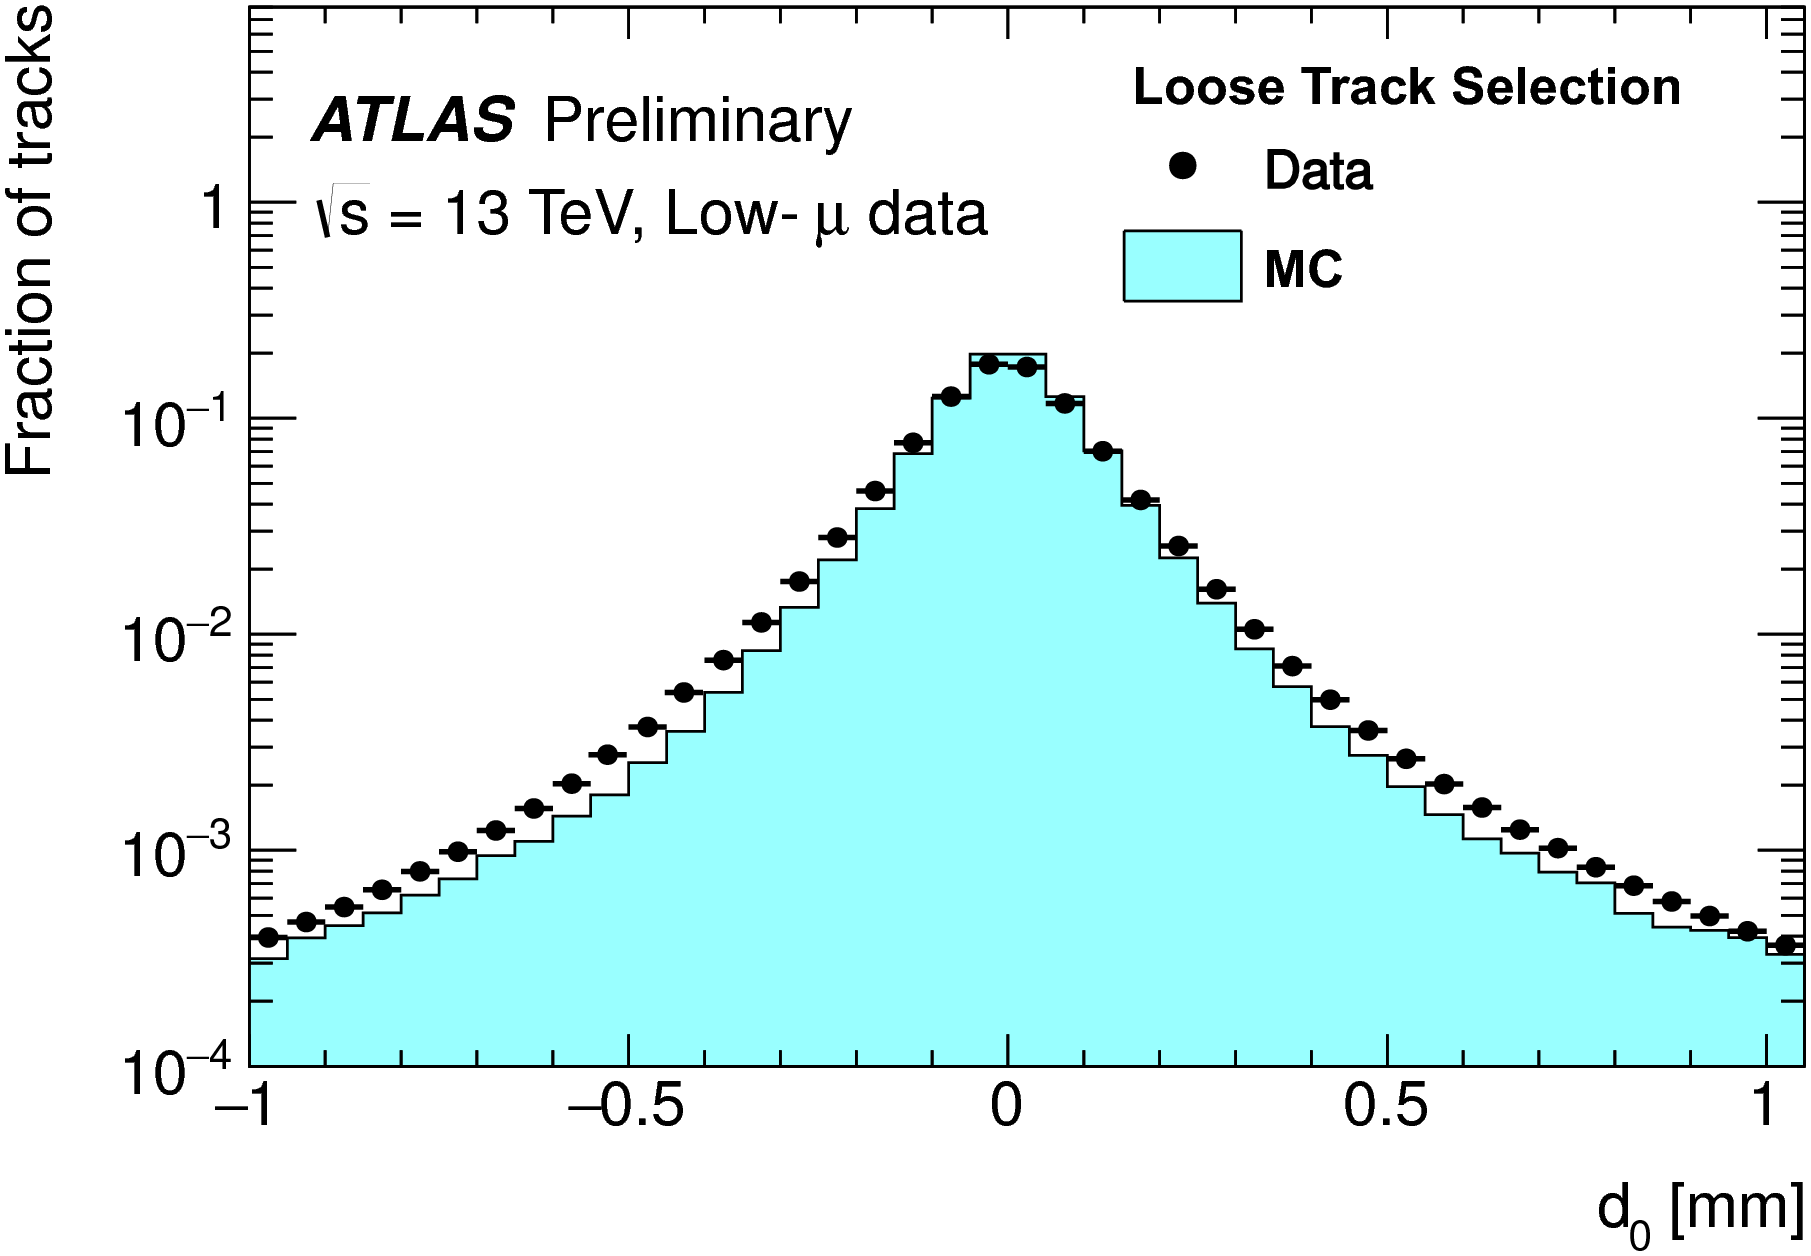
\includegraphics[width=.5\textwidth]{figures/EventReconstruction/ST-d0-eff.png}
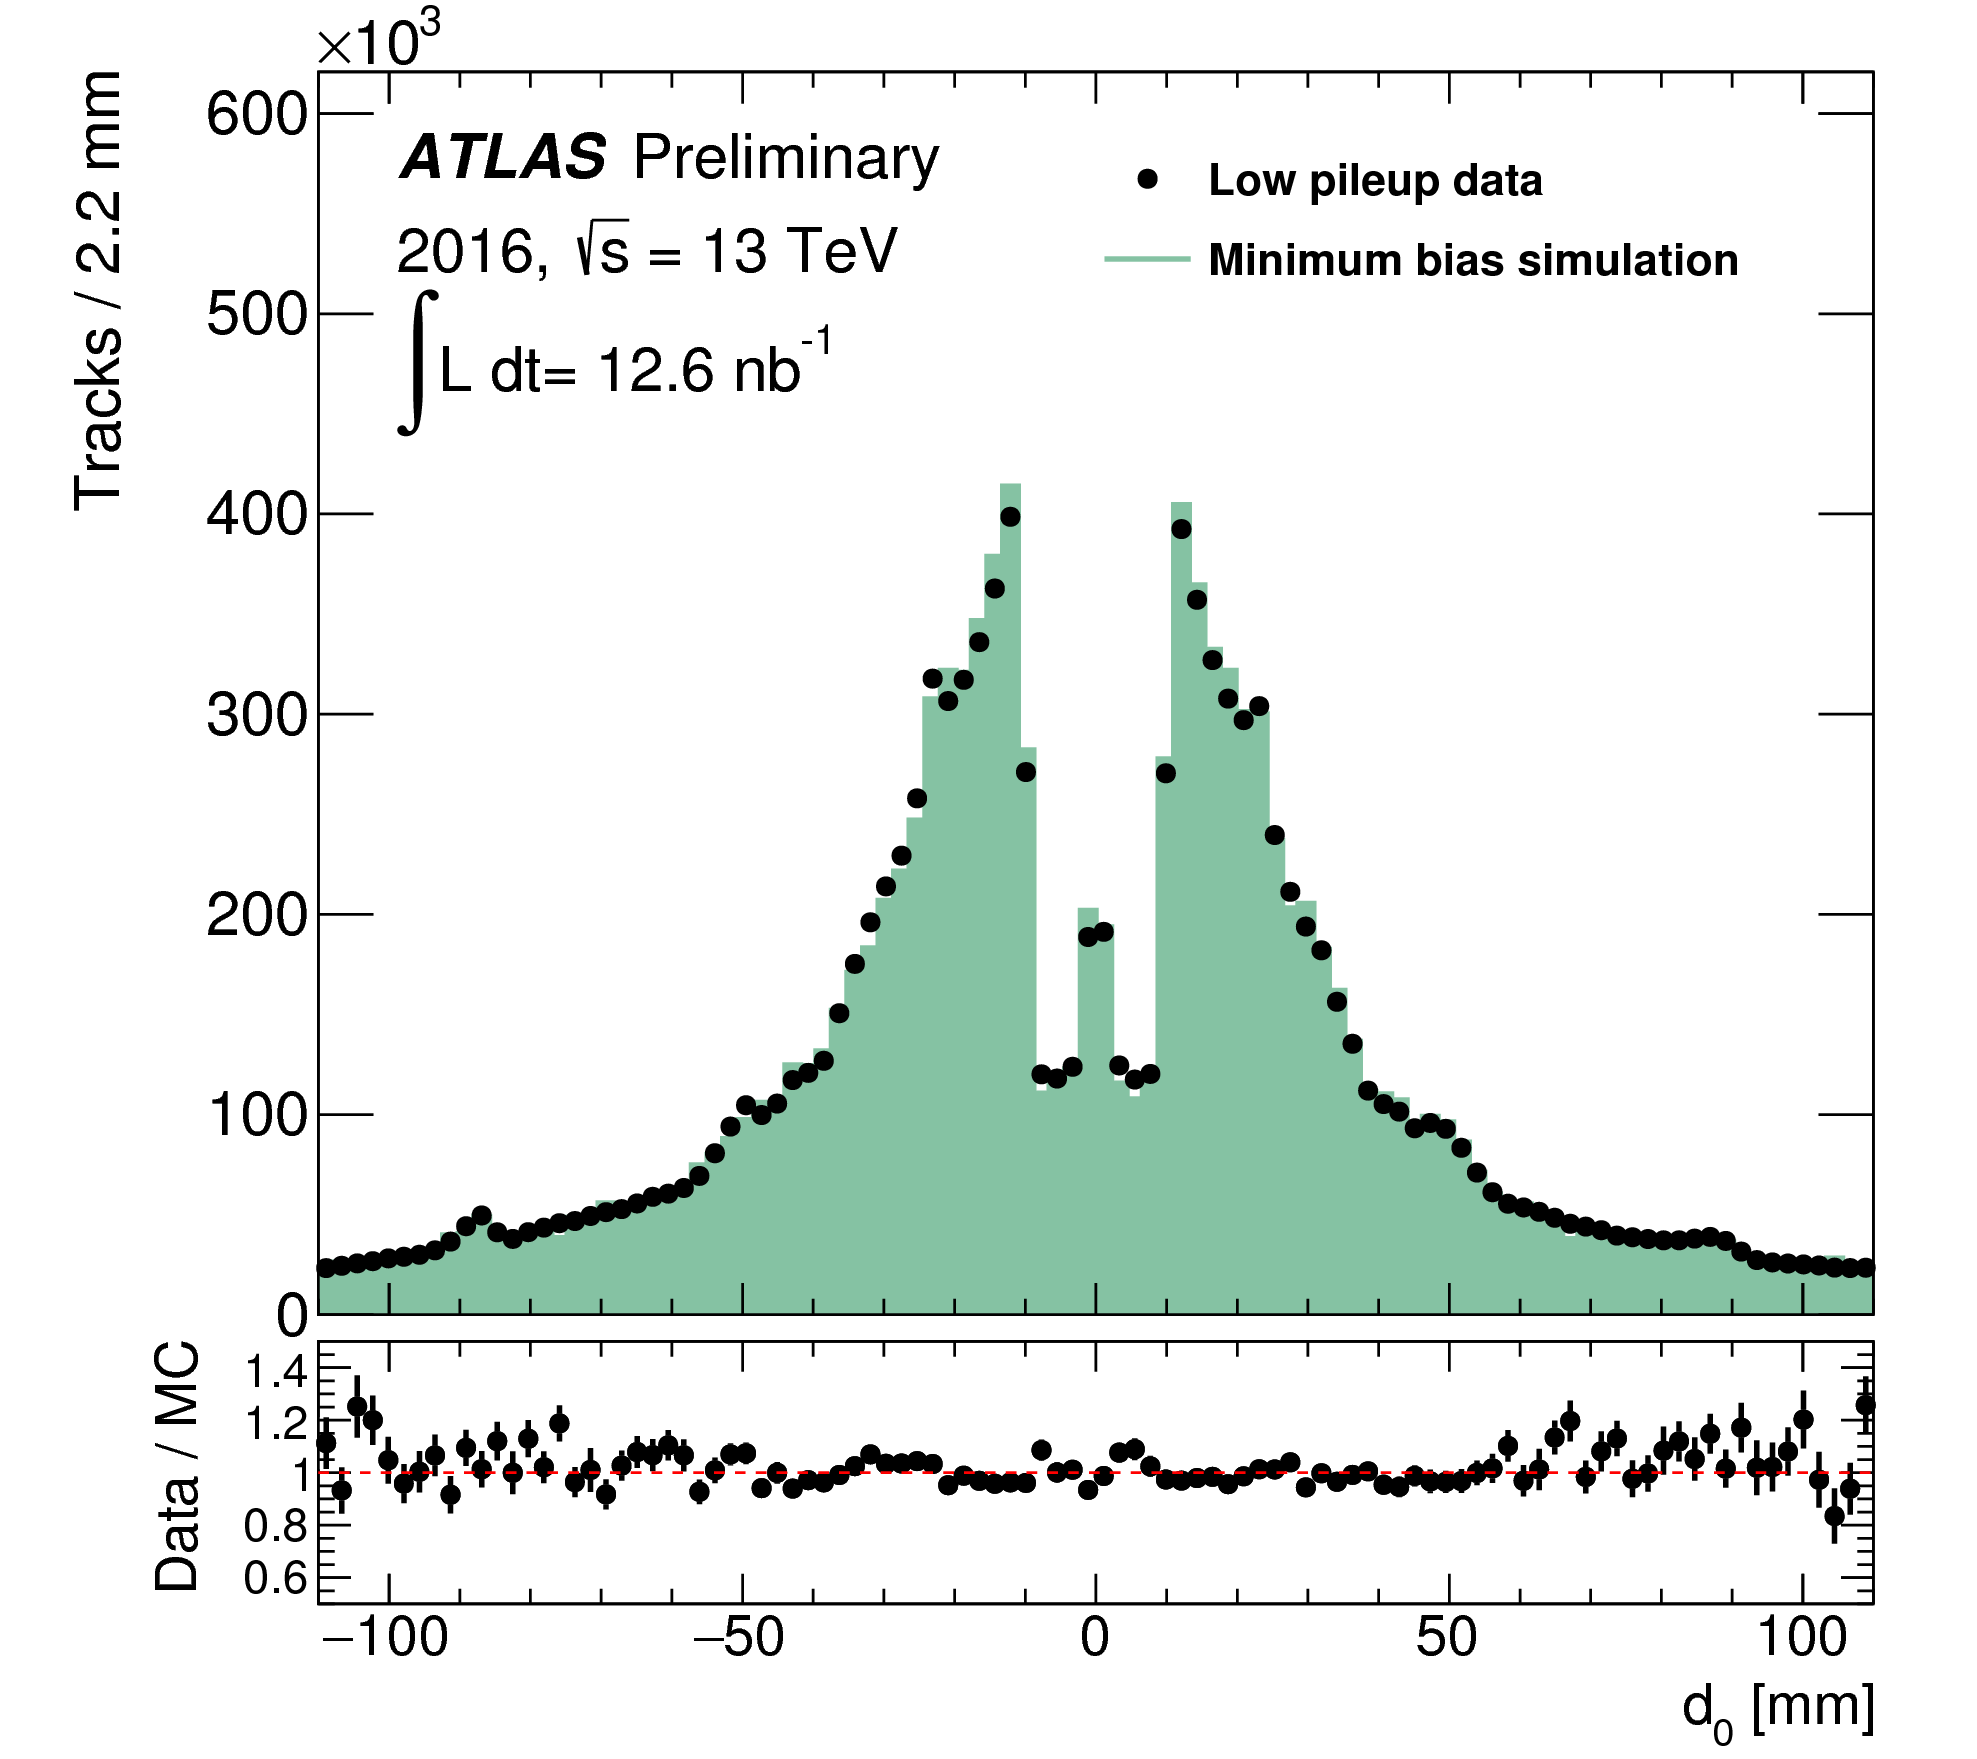
\includegraphics[width=.41\textwidth]{figures/EventReconstruction/LRT-d0-eff.png}
\caption{Number of tracks reconstructed with respect to \dzero in \ac{ST} (left) and \ac{LRT}. Note the difference in x-axis range.}
\label{fig:trking_d0_eff}
\end{figure}

\begin{figure}[htbp]
\centering
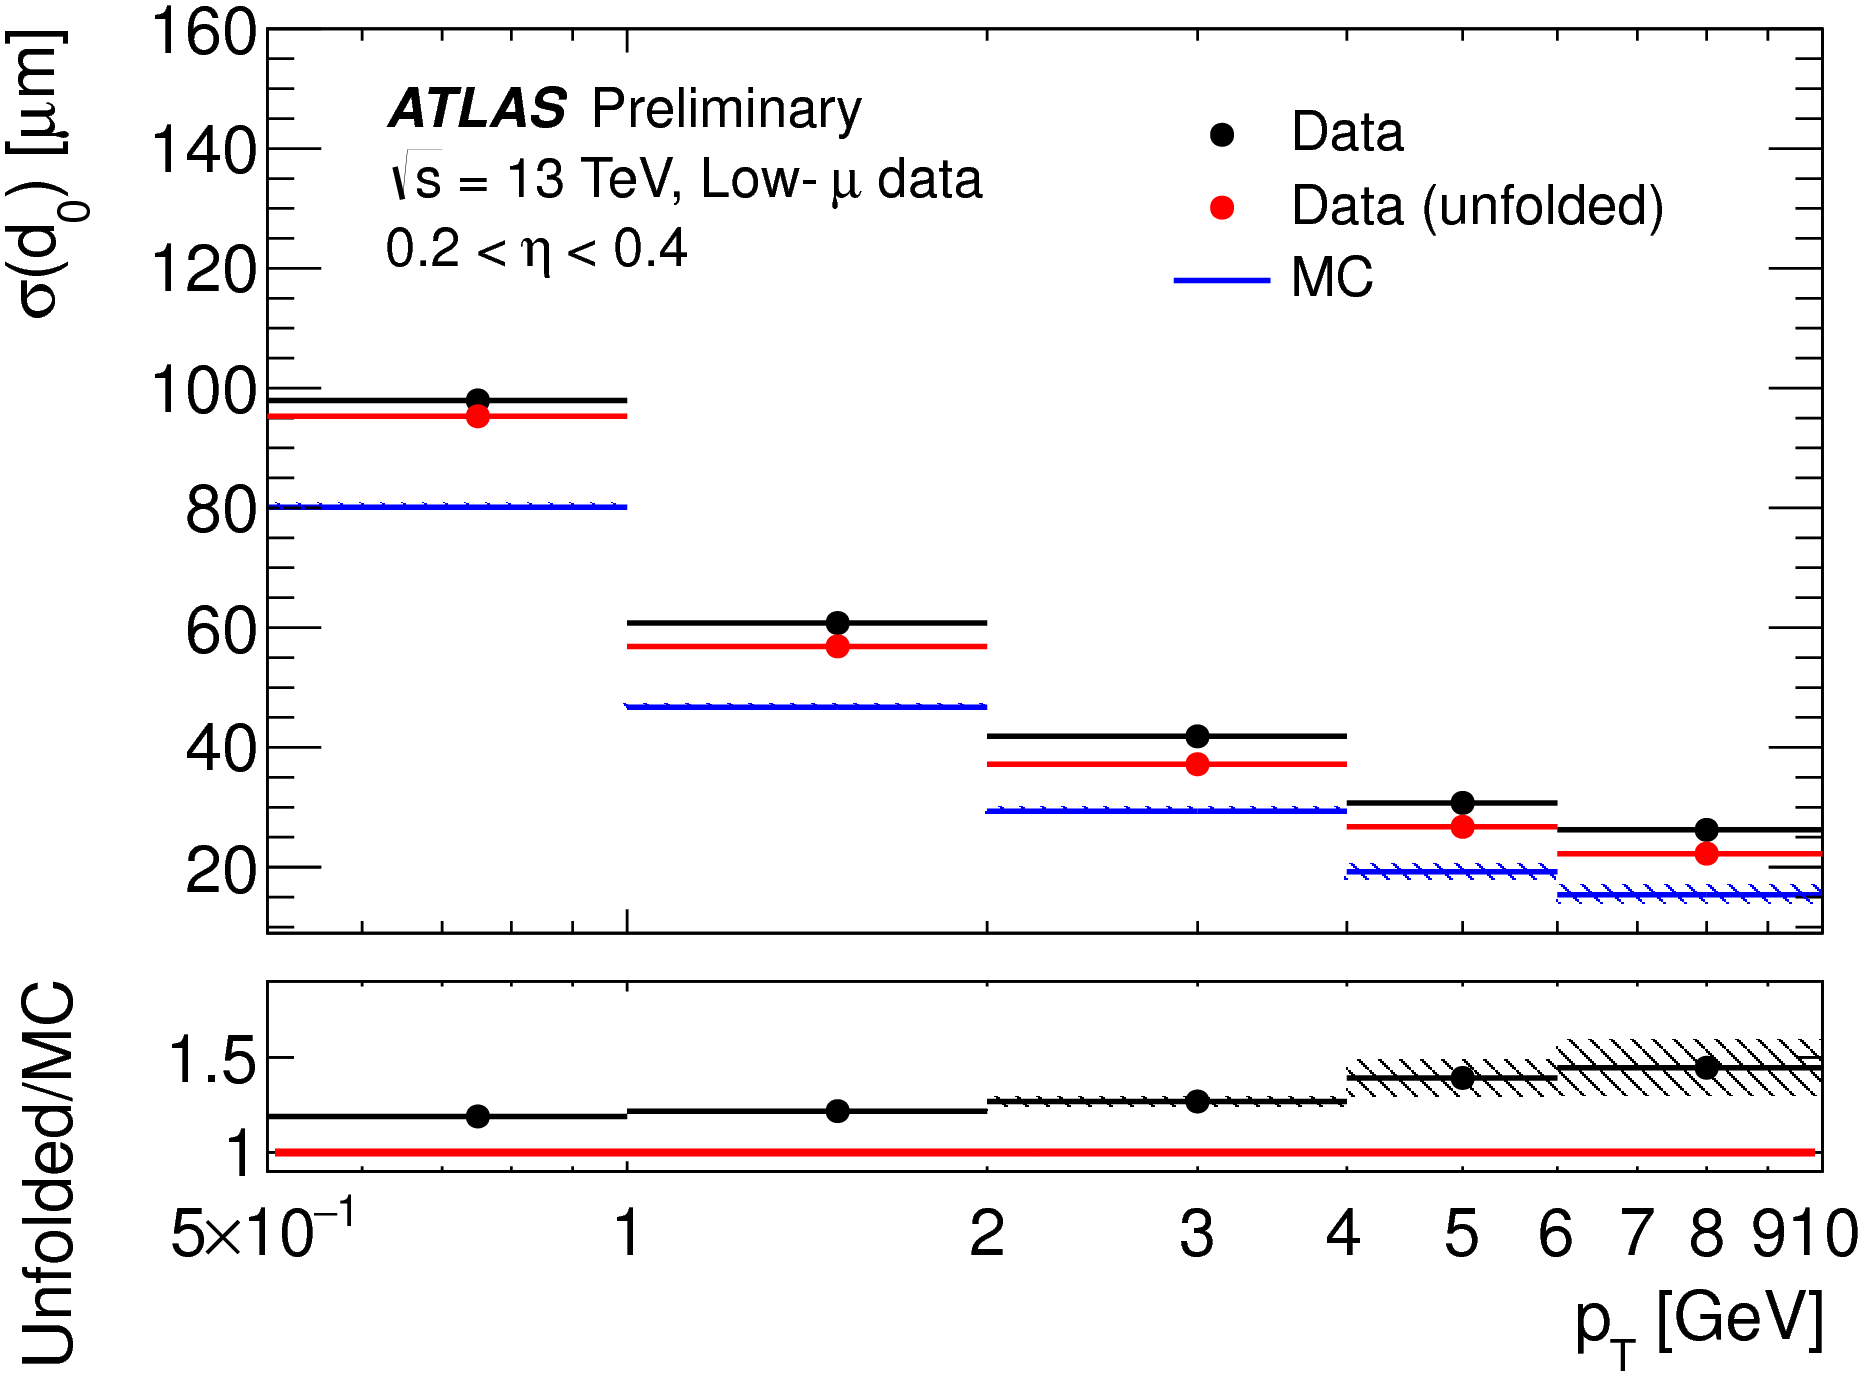
\includegraphics[width=.45\textwidth]{figures/EventReconstruction/ST-d0-res.png}
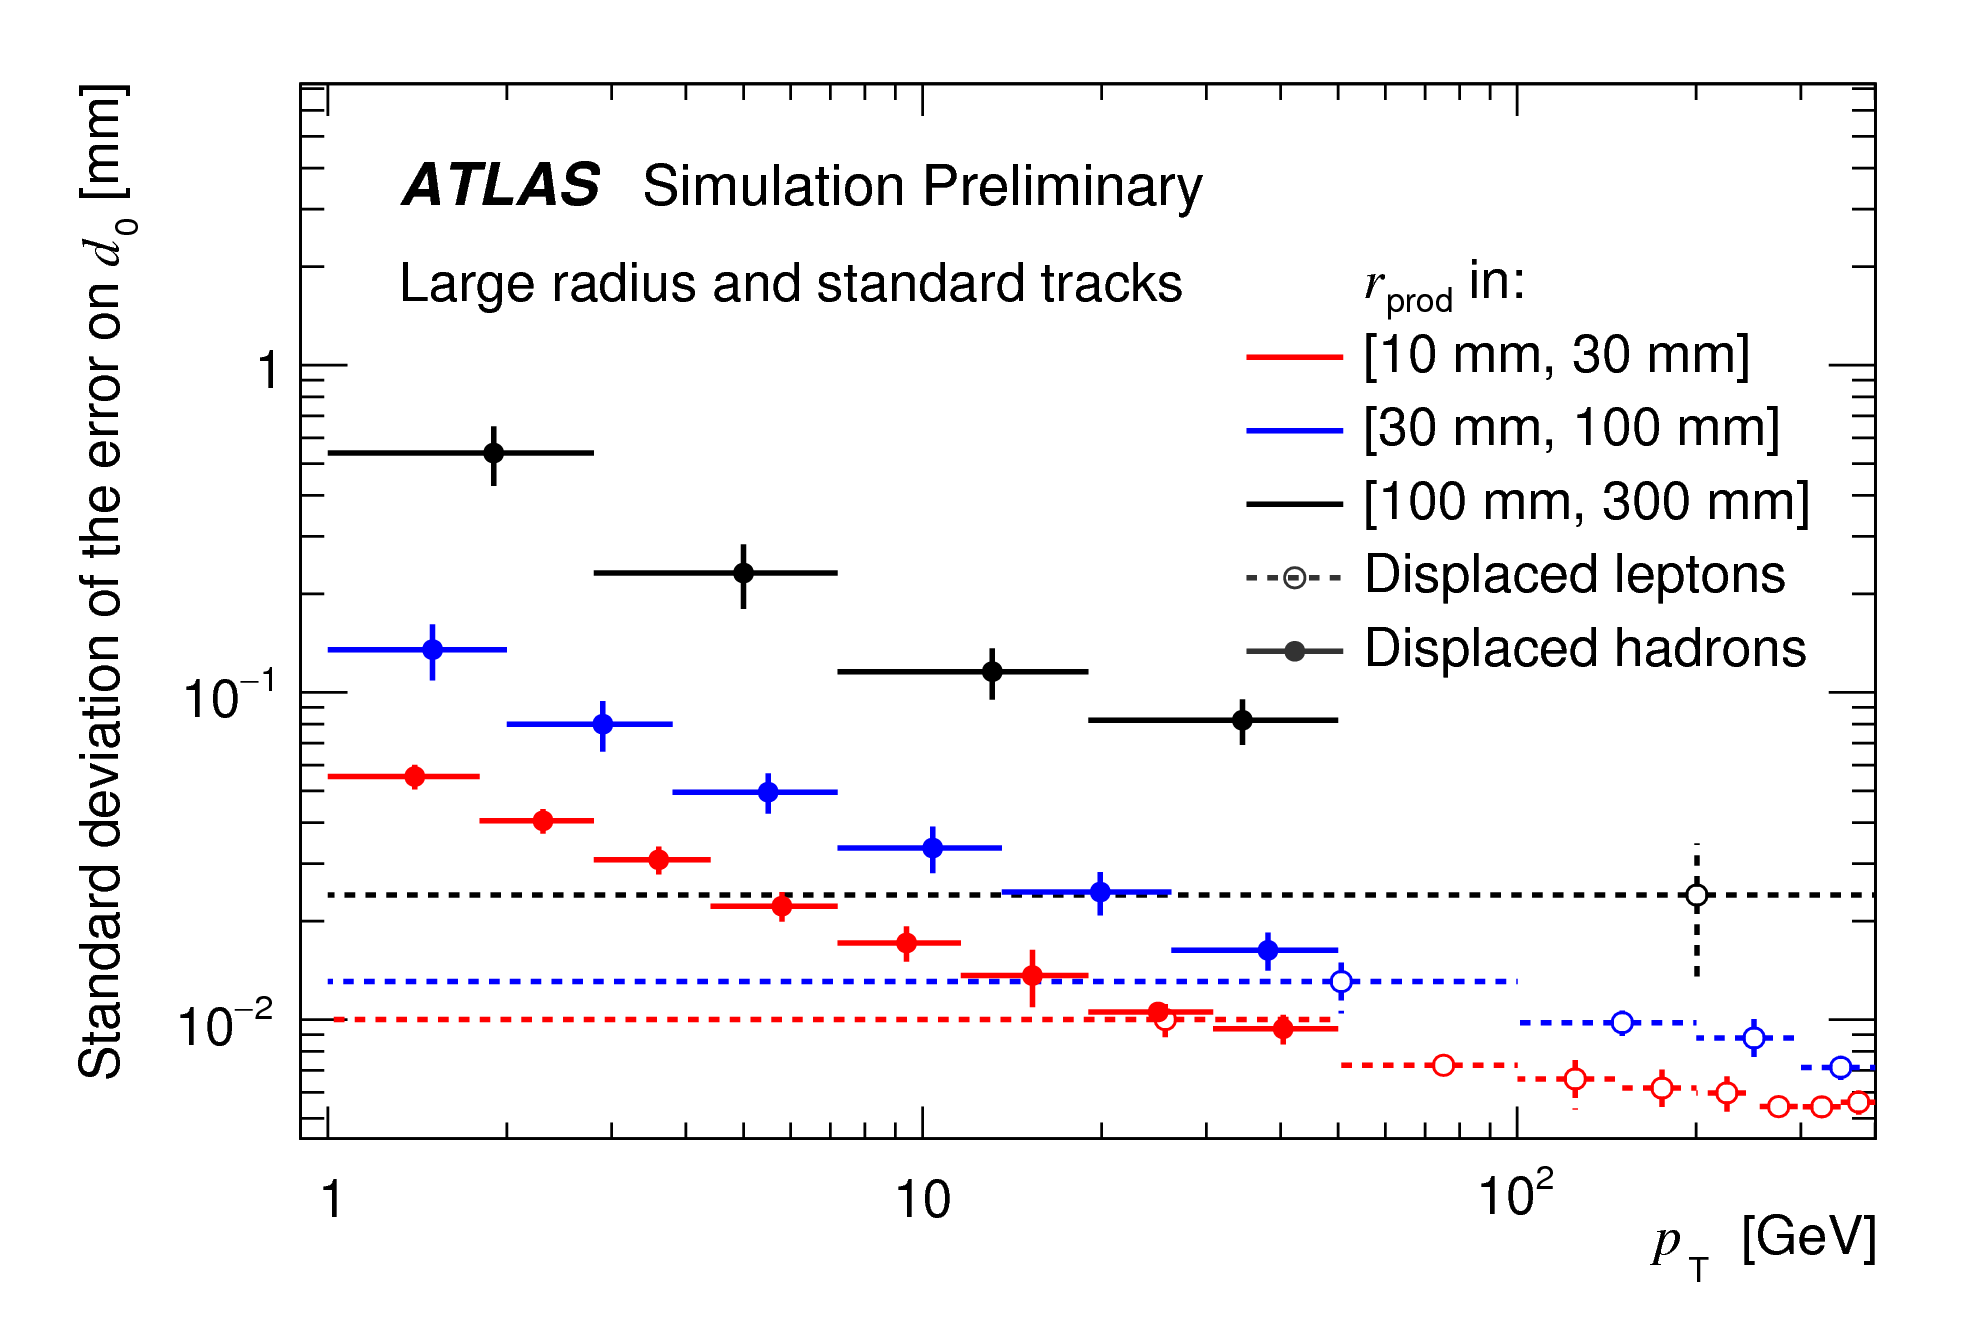
\includegraphics[width=.5\textwidth]{figures/EventReconstruction/LRT-d0-res.png}
\caption{\dzero resolution as a function of \pt in \ac{ST} (left) and \ac{LRT}. This analysis uses high \pt leptons with high \pt tracks, and thus with very good \dzero resolution}
\label{fig:trking_d0_res}
\end{figure}

%mostly used this: https://pdfs.semanticscholar.org/a591/7c383e4b07d64116b57c9c33e82138a08d12.pdf (p19+)
\subsection{Tracking Algorithms}

\subsubsection{\label{sec:kalman} Kalman Filter}

Kalman filters are widely used across LHC experiments for track fitting. It is a recursive algorithm that allows the user to efficiently extrapolate from a track seed. In the sequential, or extended, Kalman filter, uses a linear approximation to the track path. It makes a prediction for the next layer of detector material based on the seed, and then looks for a hit in that region. At each step, it updates the linearization to improve the measurement for the next step, where each measurement is weighted by its certainty. \ac{LRT} uses this approach.

In \ac{ST}, a combinatorial Kalman filter is used. This method employs several Kalman filters running in parallel and allows for the assumption that the measurement in the next layer is not necessarily assumed to be part of the track that formed the seed (as is often the case in the dense environment of the \ac{ATLAS} \ac{ID}). At each successive layer in track finding, several branches are extended if several measurements can be found in the same layer. The update of the linearization is done independently for each branch, and branches are created for missing measurements to account for detector inefficiencies. The branch is extended to the next layer if a measurement is found, and the process is repeated. Branches with no measurement for several layers are removed, and at the end, the branch with the best quality is selected. This process allows for parallelization of a complex combinatorial process. \cite{kalman-filter} 

The Kalman filter works well for tracking in environments such as \ac{ATLAS} because even though it is computationally intensive, it generally gives the best precision.

\subsubsection{\label{sec:hough} Hough Transform}

%https://indico.cern.ch/event/602049/contributions/2429704/attachments/1440531/2217489/Piucci_05_04_2017.pdf
%hough-transform.pdf

A Hough transform is a pattern recognition algorithm that is useful for identifying a particular signature that can be described in a known parametric form. It performs well in noisy environments and is tolerant of holes in the signature. In relies on a transformation from physical to parameter space. Each point in physical space maps to a line in parameter space, and the intersection of the parameter space lines gives the values of constants of the parametric form. 

For example, if the pattern being searched for is a line described by $y = mx + b$, a Hough transform maps from $x-y$ space to $m-b$ space. Each point $(x_i, y_i)$ in the original image maps to a line in parameter space. If all $(x_i, y_i)$ are plotted together, the intersections of the lines in parameter space at $(m_i, b_i)$ define lines in physical space with parameters $m_i$ and $b_i$. \cite{hough-transform}

The Hough transform is a \emph{pattern finding} algorithm, not a tracking algorithm. Is not ideal for full \ac{ID} tracking, because its complexity grows exponentially with the number of dimensions and the form of the pattern must be known \emph{a priori}.

\comebackto{How are seeds formed? Hough transform?}


\subsection{Primary Vertex Reconstruction}

After all of the tracks are reconstructed, they must be correctly assigned to a \ac{PV}. A \ac{PV} is the point in space where the $pp$ collision occurred. Generally, there are many \ac{PV}s per event: one is the hard-scatter, high-energy event of interest, and the others are pileup. In the Run 2 dataset, there are an average of 33 \ac{PV}s per event.

\ac{PV}s are reconstructed using an n iterative vertexing procedure. First, good quality tracks tracks, combined with the beamspot measurement, are used to find an optimal vertex position. Then each track is assigned a weight based on its compatibility with that position, and the vertex position is then recomputed using the weights of the tracks. After the final vertex position is determined, tracks very incompatible with the vertex are removed from it and can be used to create another vertex. Any vertex with at least two tracks are considered \ac{PV}s.



%-----------------------------
% Muon Reconstruction
%-----------------------------
\section{Muons}
%USED atlas-muon-reco.pdf
\label{sec:muonreco}
\subsection{Standard Reconstruction and Identification}

Muons are reconstructed by combining a \ac{MS} track with an \ac{ID} track. Then, at the identification stage, quality requirements are imposed on the combined tracks to improve the purity of the muon collection. For this analysis, the muon reconstruction algorithm remains unchanged (though \ac{LRT} tracks are used), while changes are made at the identification stage. \cite{muon-reco}

\subsubsection{Muon Track Reconstruction}
To reconstruct \ac{MS} tracks, a Hough transform (described in \autoref{sec:hough}) is used to search for hits in each \ac{MDT} chamber to find hits following a trajectory on the $\eta$ plane of the detector. These hits are fit to a straight line within each chamber to form \emph{segments}. Co-located \ac{RPC} and \ac{TGC} hits are used to measure the $\phi$ coordinate. 

Hits from segments in various layers are fit to form track candidates. This fitting is first seeded from segments in the middle layers of the \ac{MS} where more trigger hits are available, then extrapolated inward and outward. A next pass is done using inner and outer station segments as seeds. The extrapolation relies on relative positional and angular information, as well as the fit quality and hit multiplicity of the segments. Two segments are required to make a track, except in regions with limited detector coverage, where one high quality segment is sufficient. After all extrapolation, an overlap removal procedure is performed, allowing for a segment to be shared between at most two tracks. A $\chi^{2}$ test is performed, where outliers hits can be removed from the track and additional hits consistent with the track candidate's trajectory can be added.

\comebackto{what are "trigger hits"}


\subsubsection{Combined Muons}
Next, the \ac{MS} tracks are combined with \ac{ID} tracks to form \ac{CB} muons, a track fit over the two tracks. \ac{CB} muon tracks are generally seeded from the \ac{MS}, then extrapolated inward and matched to an \ac{ID} track, but the inverse is also allowed. Hits from the \ac{MS} may be added or removed to improve the fit between the two tracks.



\subsubsection{Muon Identification}

This analysis uses the default muon working point for ATLAS analyses, called a \emph{medium} muon. This working point places a requirement on the number of \ac{ID} and \ac{MS} hits that comprise the track to ensure a robust momentum measurement. At least 1 pixel hit, at least 5 \ac{SCT} hits are required and at least 10\% of the \ac{TRT} hits associated to the object must be included in the final fit. There must also be fewer than 3 holes in the silicon tracking layers. Furthermore, the \ac{MS} track must have at least 3 hits in at least 2 \ac{MDT} layers. In the crack region $|\eta| < 0.1$, \ac{MS} tracks with at least three hits in only one \ac{MDT} layer are allowed provided there are no holes in the track. Finally, a loose requirement is placed on the consistency between the \ac{MS} and \ac{ID} tracks. Namely, the \emph{q/p significance}, the difference between the charge and momentum ratio in the \ac{ID} and \ac{MS} divided by their uncertainties summed in quadrature, is required to be less than 7. 


\begin{figure}[htbp]
\centering
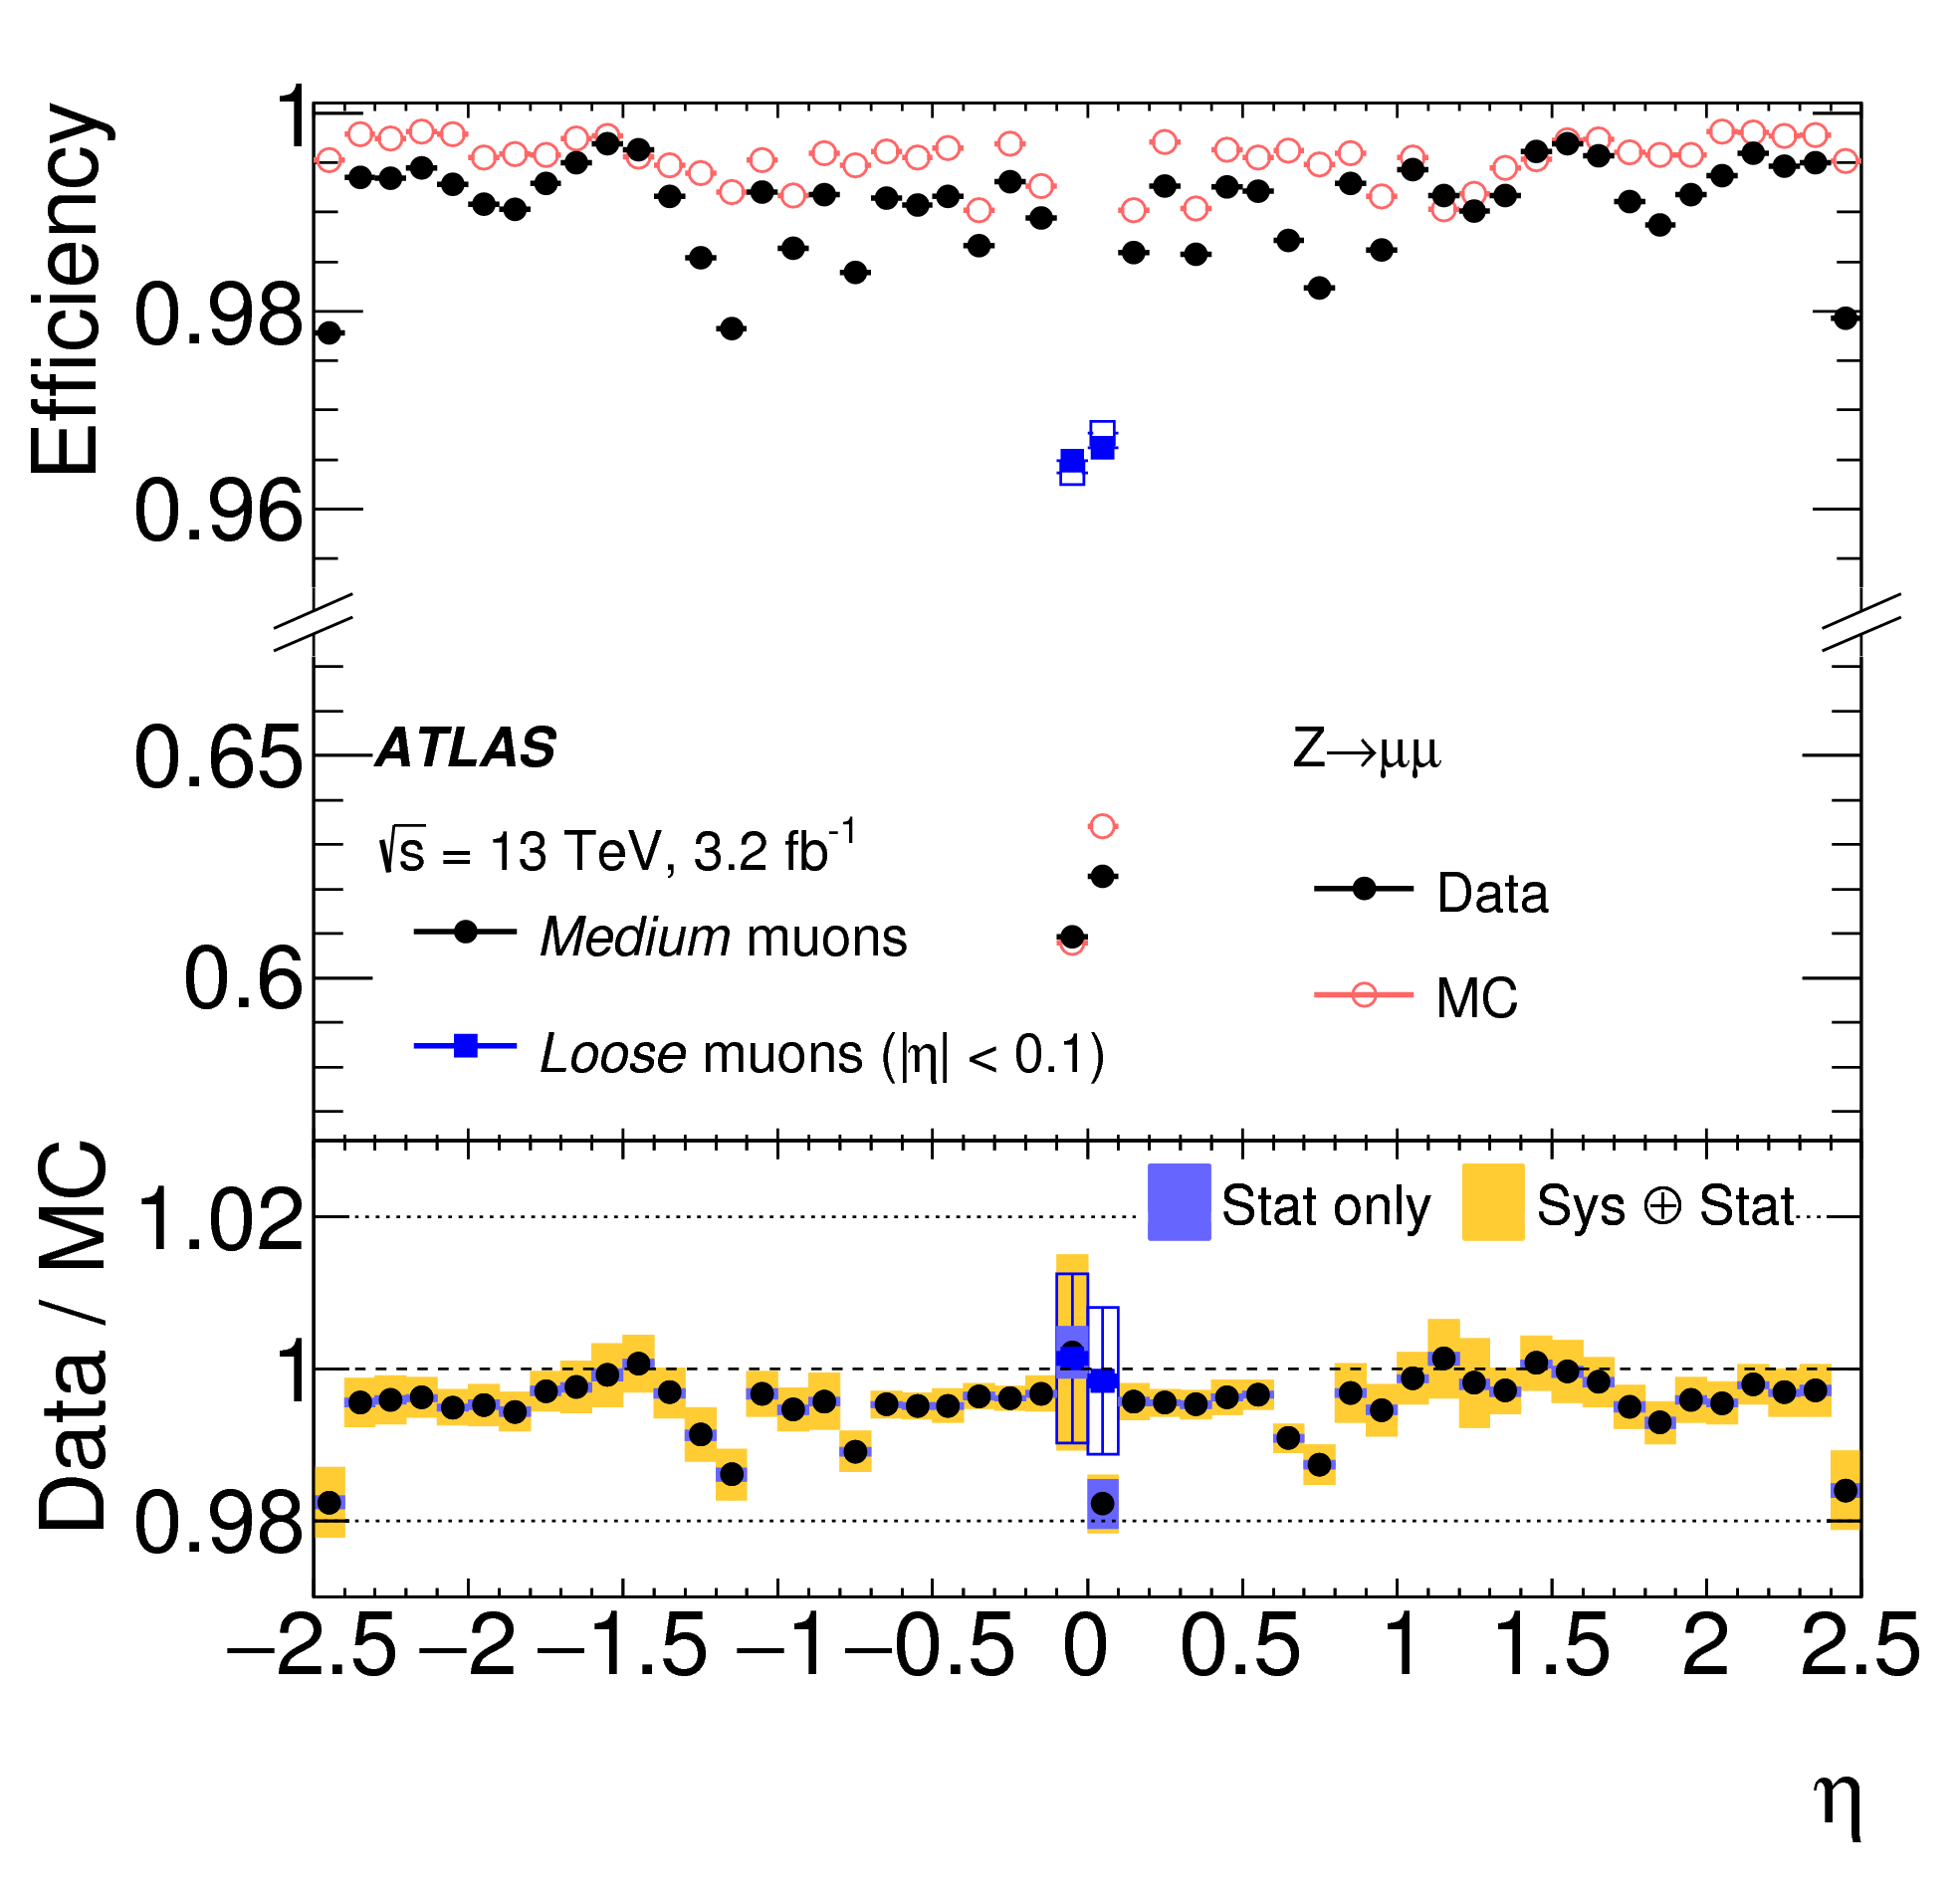
\includegraphics[width=.43\textwidth]{figures/EventReconstruction/muon-reco-eta.png}
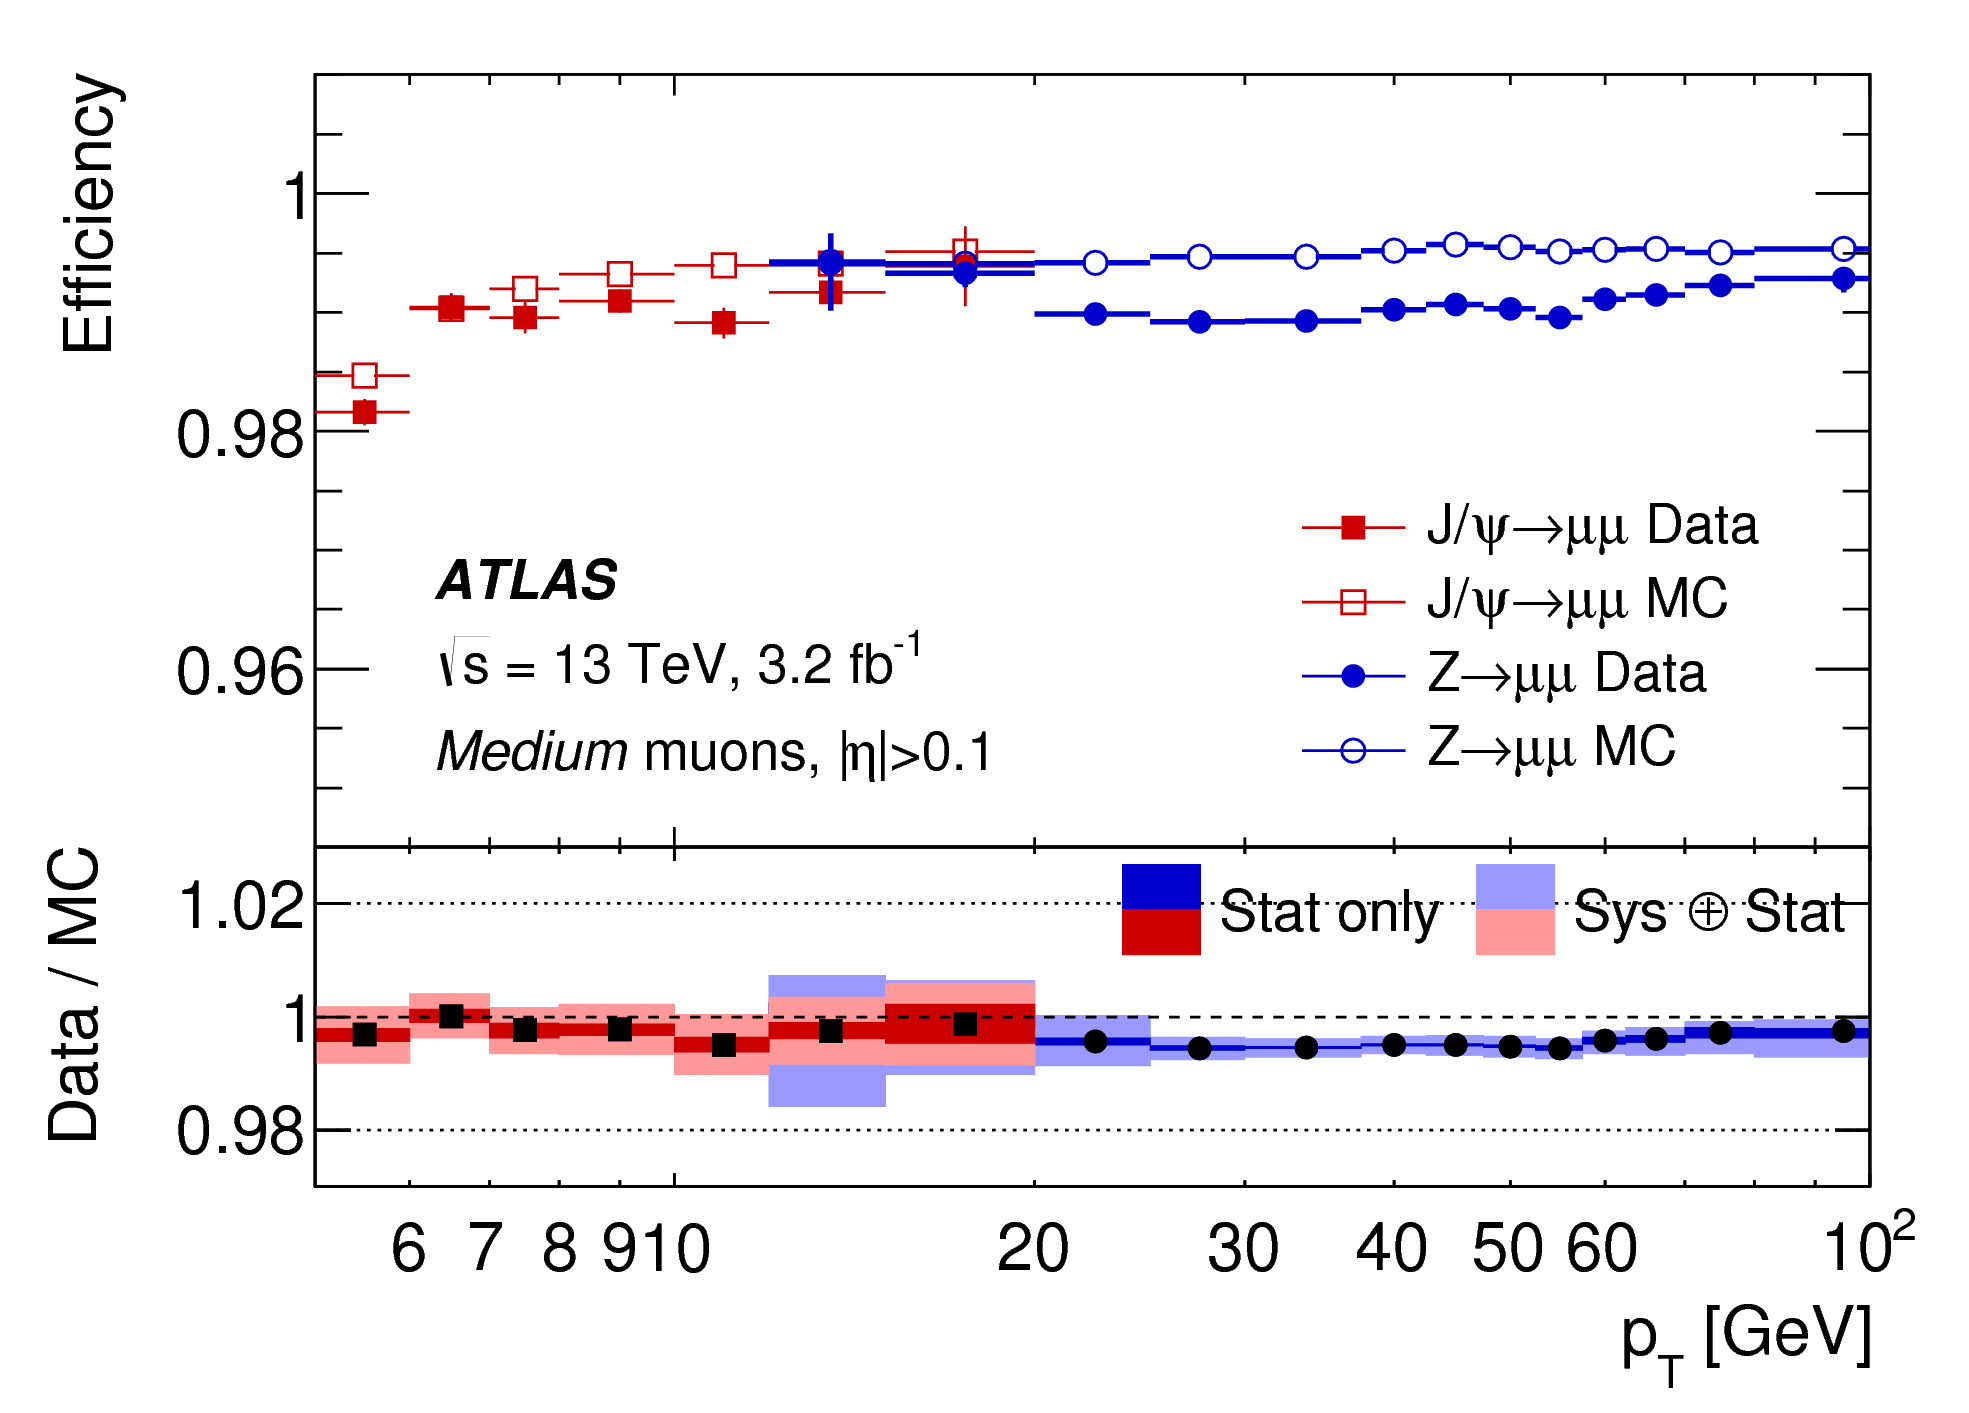
\includegraphics[width=.52\textwidth]{figures/EventReconstruction/muon-reco-pt.png}
\caption{Medium muon identification efficiency with standard tracking and criteria. Left is efficiency vs $\eta$ and right is efficiency as a function of $p_{T}$. Medium muons are reconstructed very efficiently, except for around $|\eta| \approx 0$, where the \ac{MS} is missing detector coverage.}
\label{fig:std_muon_eff}
\end{figure}


\subsection{Modifications}
\label{sec:mu_reco_mods}

For this analysis, muons are reconstructed after \ac{LRT} is performed and the reconstruction and identification efficiency is quite high. Furthermore, at the identification stage, we remove the requirement that the \ac{ID} track has at least one pixel hit, further improving the efficiency at high $d_{0}$. The effect of these improvements is show in \autoref{fig:cust_muon_eff}


This modification of the muon identification increases the fake rate of muons, so again we impose quality requirements that are independent of displacement. We require the muon to have at least two \ac{MS} layers with at least three precision hits, that the muon have at least one $\phi$ measurement (otherwise the \ac{MS} $\phi$ measurement is taken as the center of the \ac{MDT}, with an uncertainty of 0.2) and require the $\chi^{2}_{CB}/N_{DoF} < 3$. The $\chi^{2}_{CB}$ requirement is, in effect, a requirement on the consistency between the the \ac{ID} and \ac{MS} tracks. These will be further discussed in \autoref{sec:mu_qual_req}


\begin{figure}[htbp]
\centering
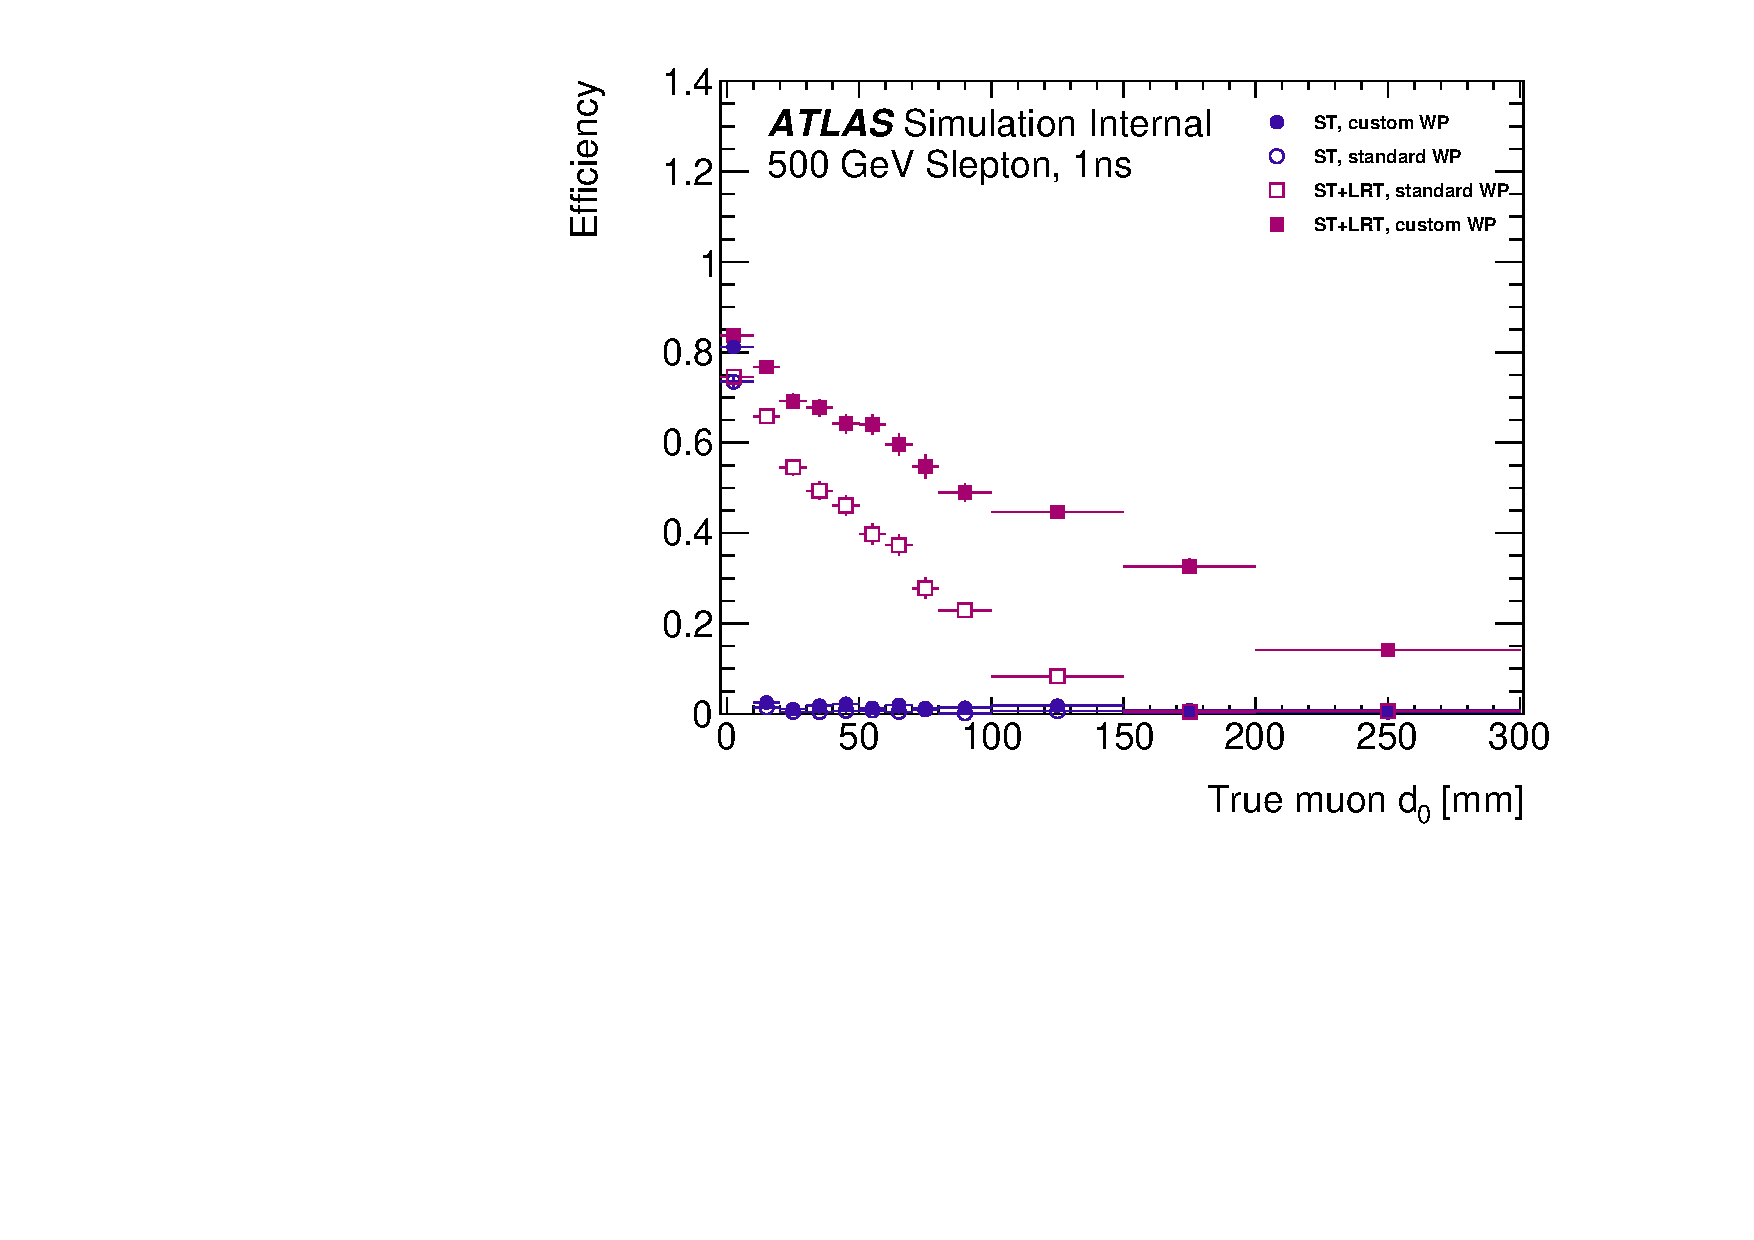
\includegraphics[width=.48\textwidth]{figures/EventReconstruction/wp_m_d0_all_wip.pdf}
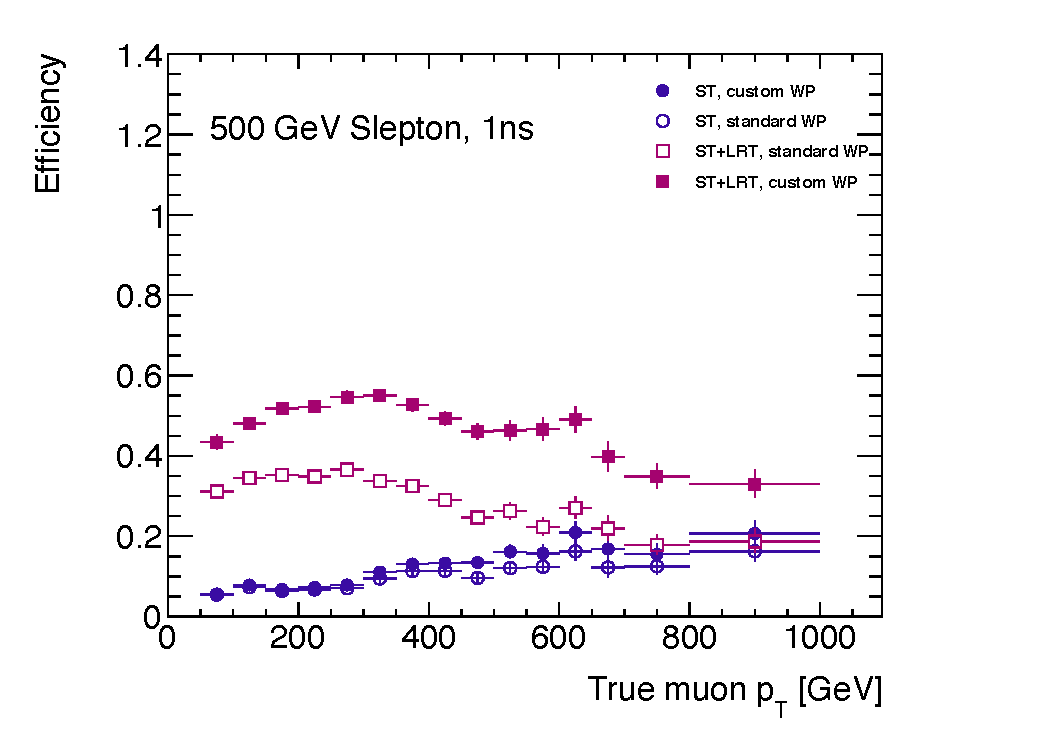
\includegraphics[width=.48\textwidth]{figures/EventReconstruction/wp_m_pt_all_wip.pdf}
\caption{Muon identification efficiency with modified criteria. Left is efficiency vs $d_{0}$ and right is efficiency as a function of $p_{T}$. The red denotes reconstruction with Standard Tracking (ST), and the blue with Large Radius Tracking (LRT), and the filled in circles use the modified identification working point. \todo{Needs update when available}}
\label{fig:cust_muon_eff}
\end{figure}



%-----------------------------
% Electron Reconstruction
%-----------------------------
\section{Electrons}
%USED atlas-electron-reco.pdf atlas-electron-reco-sliding-window.pdf
\label{sec:elecreco}

Electrons are reconstructed using clusters from the \ac{EM} calorimeter as well as tracks from the \ac{ID}. \cite{electron-reco} Electron reconstruction brings more complication and ambiguity than muon reconstruction because of the presence of photons, converted photons, and bremsstrahlung radiation from electrons moving through material. These factors make the identification and accurate measurement of electrons quite challenging. More than in muon reconstruction, it relies on displacement-based quality information, posing a problem for this search. We modify these requirements and use \ac{LRT} tracks, but have a resulting lower selection efficiency. 

\subsection{Standard Reconstruction and Identification}


\subsubsection{Cluster Reconstruction}

First, clusters are formed from $\eta \times \phi$ \emph{towers} of size $\Delta \eta \times \Delta \phi = 0.025 \times 0.025$ (roughly granularity of the second layer of the \ac{EM} calorimeter, where about 80\% of the energy in a shower is deposited). In each region, the energy deposited in all layers of the calorimeter is summed and are used as input to a seeding algorithm to form clusters. 

A \emph{sliding window} algorithm \cite{electron-sliding-window} is used to form clusters. In this algorithm, an $3 \times 5$ window is slid across each tower, the energy is summed inside of this window. If the sum is a local maximum and is above a threshold of $\et > 2.5 \GeV$, this window is considered a \emph{cluster}. A duplicate removal process is then performed for nearby clusters with similar energy measurements, keeping only the cluster with the largest $E_{T}$. Inefficiency in the cluster reconstruction step is negligible compared to the uncertainty in the next two steps. The efficiency of this step is 65\% at $\et = 4.5 \GeV$ and $> 99\%$ above $\et = 15 \GeV$.

\begin{figure}[htbp]
\centering
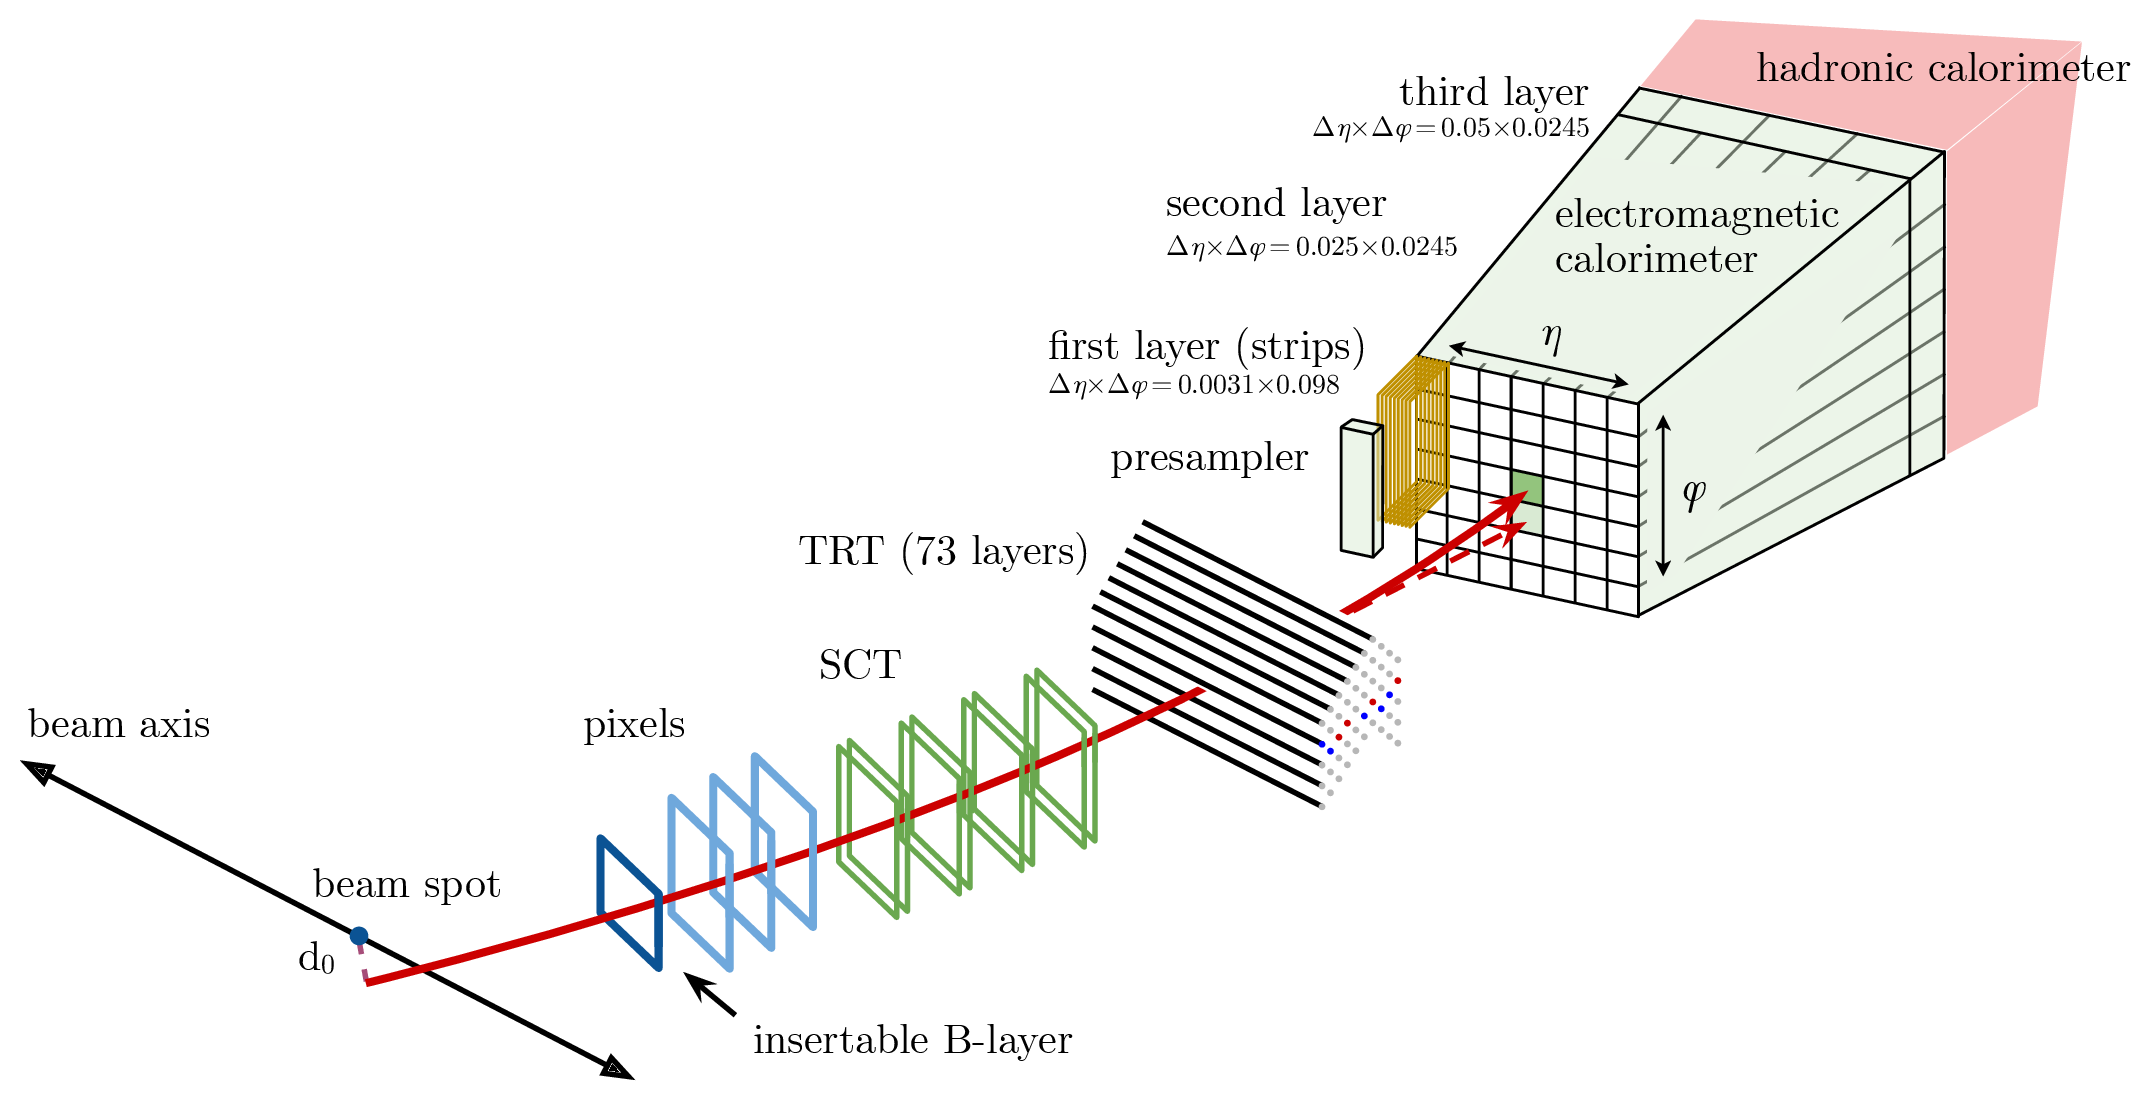
\includegraphics[width=.8\textwidth]{figures/EventReconstruction/electron-reco-sketch.png}
\caption{A sketch of an electron's path through a slice of the \ac{ATLAS} detector.}
\label{fig:elec_reco_sketch}
\end{figure}

\subsubsection{Tracking}
Since electrons are so light, they can lose a significant amount of their energy due to bremsstrahlung radiation as they traverse the \ac{ID}, thus resulting in a track seed that cannot be extended to the requisite number of silicon layers using the processes described in \autoref{sec:trackreco}. Thus, a second pass at tracking, allowing for 30\% energy loss due to bremsstrahlung radiation at each detector layer is performed in the vicinity of a good quality \ac{EM} cluster. Here, the track candidate $p_{T}$ is lowered to $400 \MeV$ (compare to $1 \GeV$), but still uses the standard hypothesis that the track is like that from a pion. If this fit still fails, a third pass is performed using the assumption that the track is like that from an electron, allowing for an additional degree of freedom in the $\chi^2$ calculation that accounts for additional radiation. In all, this gives 98\% reconstruction efficiency for electrons with $\et > 10 \GeV$. 

This loosened track fitting requirements allow for increased efficiency, but the resulting tracks do not correctly account for the energy loss of the electron to the material. An additional tracking pass, using an optimized \ac{GSF} is used to correct for this. 

This procedure is performed on tracks with at least 5 silicon hits and roughly match to an \ac{EM} cluster. The \ac{GSF} procedure is based on a combinatorial Kalman filter, resulting in track parameters weighted by Gaussian function describing material-induced energy losses. This procedure also accounts for the increase in curvature caused by the decrease in momentum due to energy loss in material, improving the calculation of track parameters. An example of this is show in the figure below. The reconstruction efficiency for this step is around 98\% for electrons with $\et > 30 \GeV$. 

\begin{figure}[htbp]
\centering
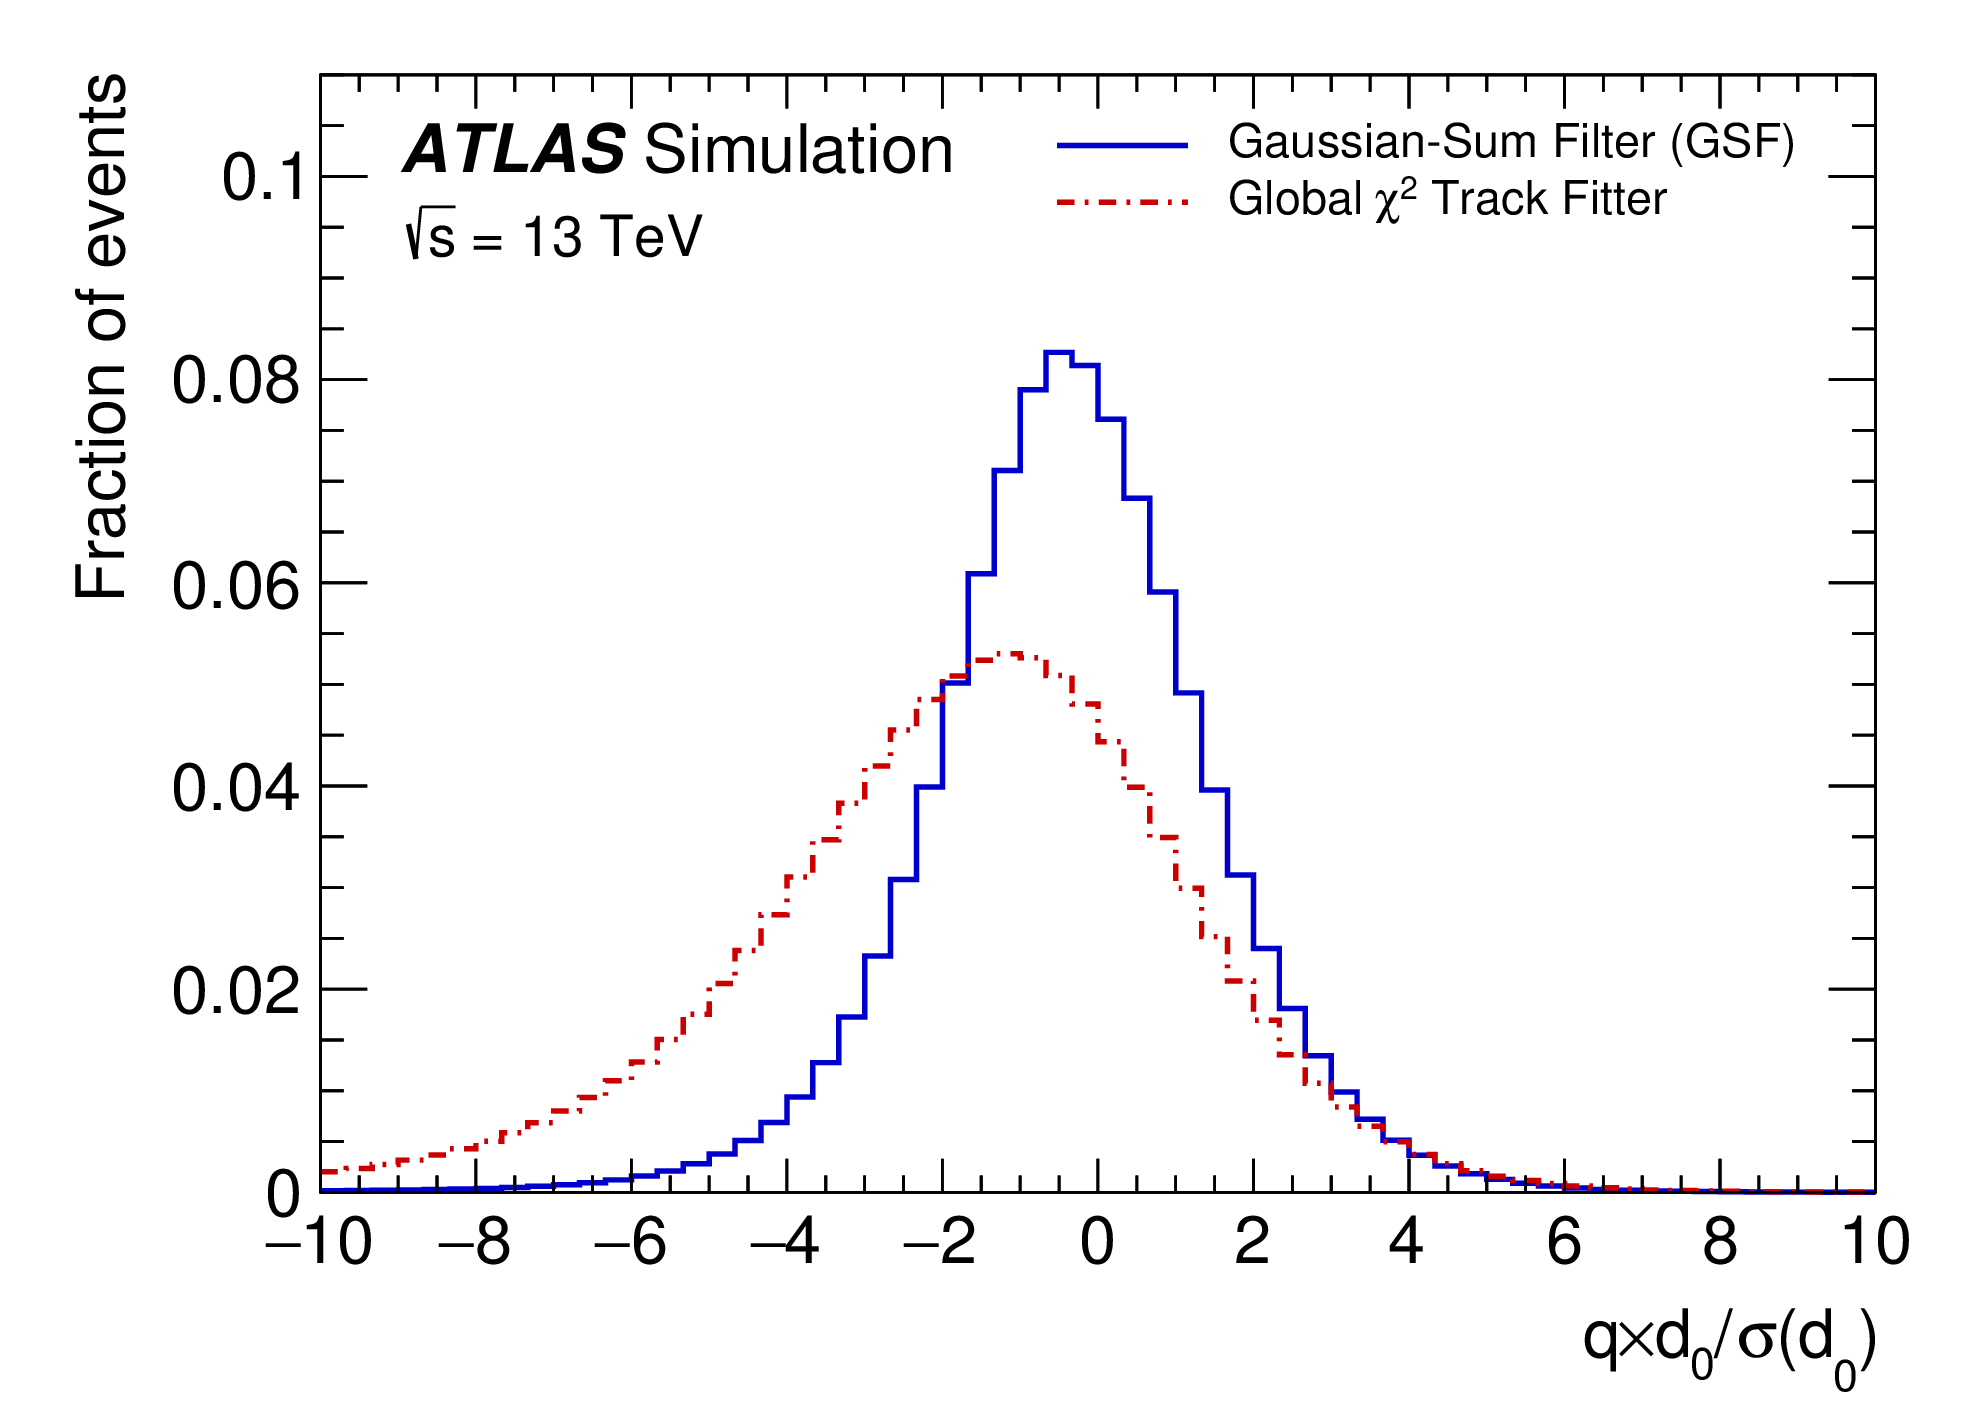
\includegraphics[width=.7\textwidth]{figures/EventReconstruction/elec-qxd0.png}
\caption{The impact on the $q \times \dzero /\sigma(\dzero)$ measurement by the addition of \ac{GSF} tracking. This is sampled from prompt electrons, so the narrower distribution centered around zero indicates significant improvement.}
\label{fig:elec_gsf}
\end{figure}


\subsubsection{Combined Reconstruction}
To put it all together, \ac{GSF} tracks are then matched to seed calorimeter clusters then the final cluster size is determined. Tracks and clusters are matched with stricter requirements, requiring that their $\phi$ measurement is within $+0.05$ or $-0.10$. It is possible that several tracks might match to the same cluster, but a primary track is assigned based on its proximity and quality. If the track can be associated to a vertex, it is classified as a potential photon conversion, not an electron. Electrons are further distinguished from photon conversions using their $E/p, p_{T}$, and number of pixel hits. 

Final clusters are formed by looking in a window around the seed cluster. The reconstructed electron's energy measurement is taken from its full cluster, and directional information taken from its track. At $\et > 15 \GeV$, there is a 99\% efficiency to reconstruct an electron (provided it has at least one pixel hit and at least seven total silicon hits on track). 

\begin{figure}[htbp]
\centering
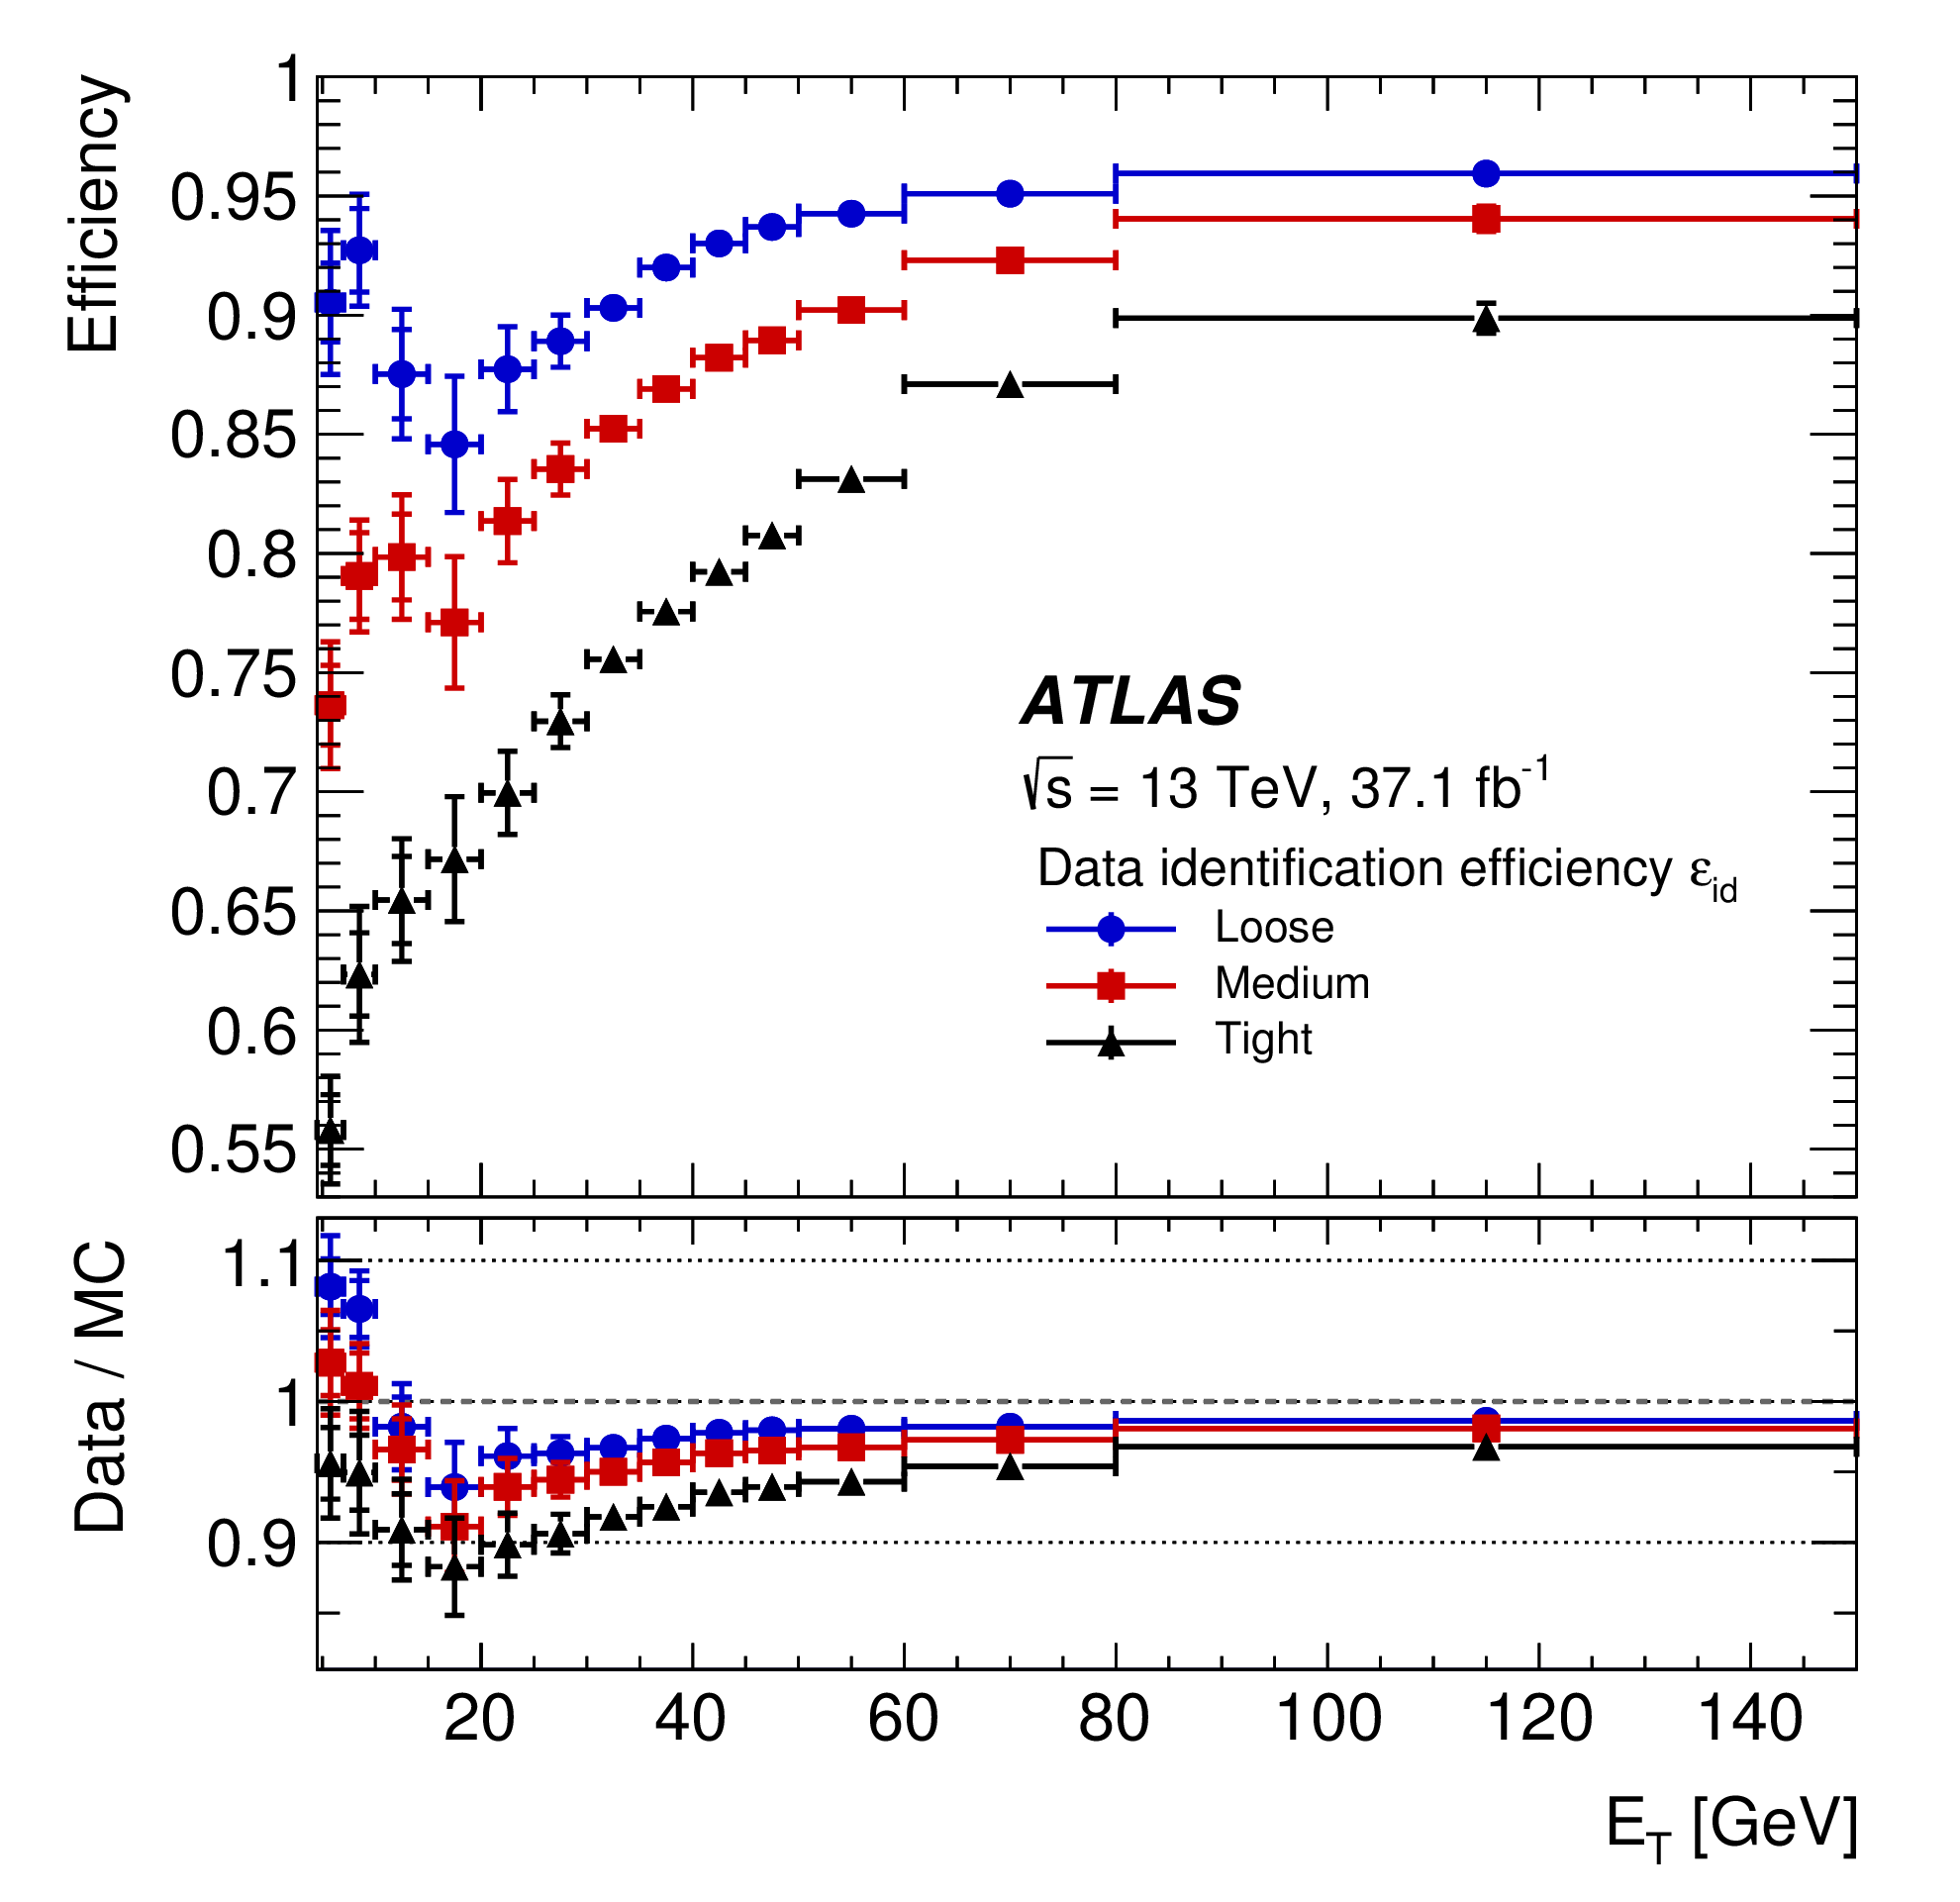
\includegraphics[width=.4\textwidth]{figures/EventReconstruction/elec-reco.png}
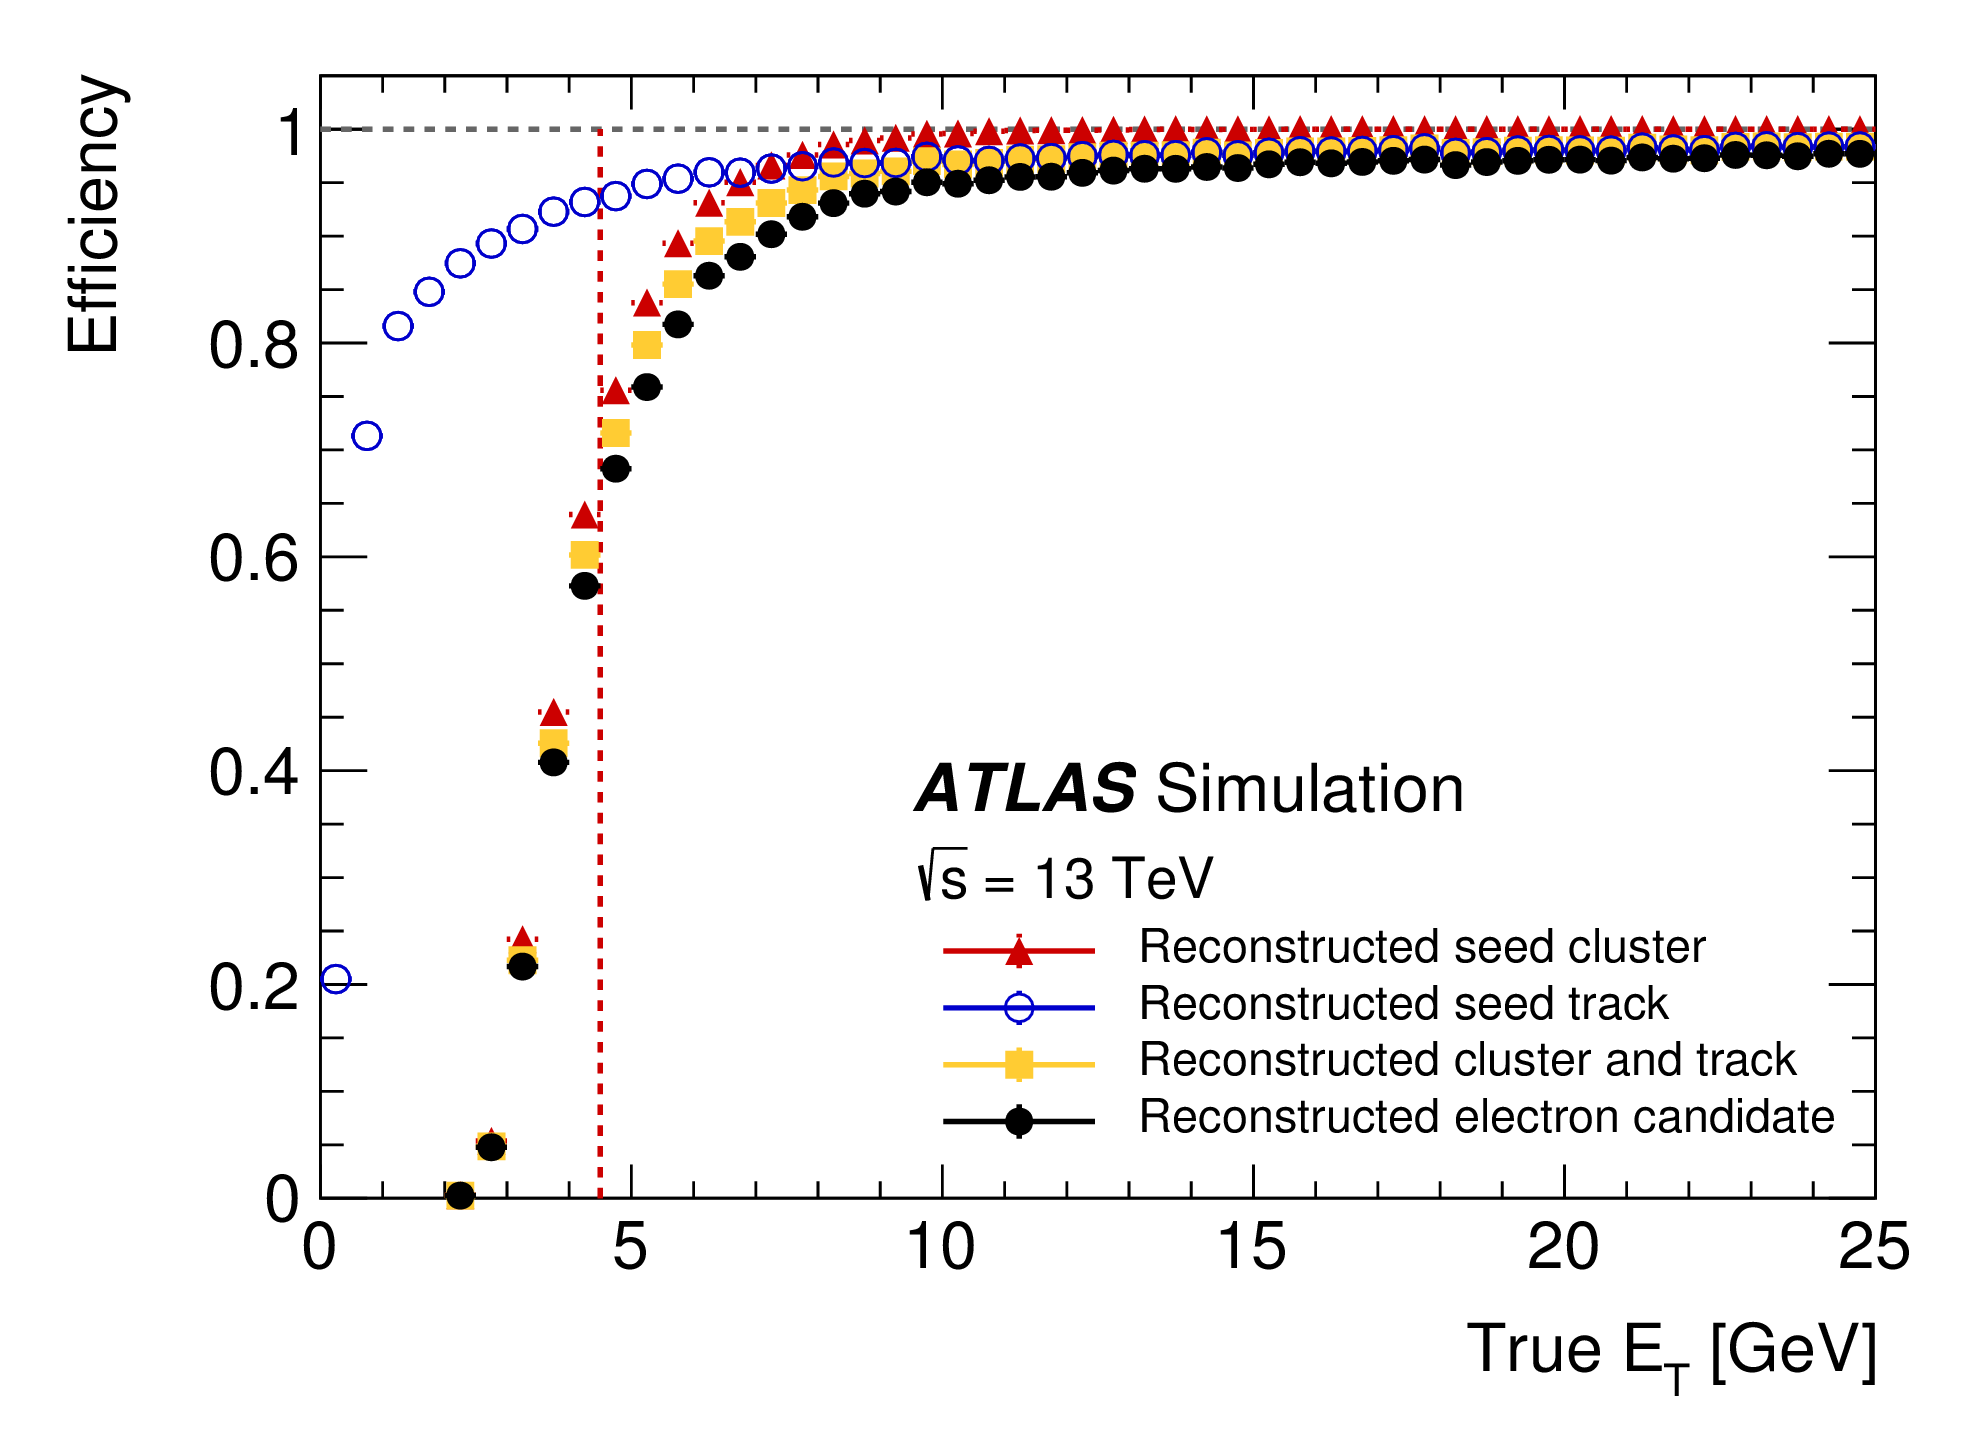
\includegraphics[width=.5\textwidth]{figures/EventReconstruction/elec-reco-steps.png}
\caption{Electron reconstruction efficiency as a function of true transverse energy, \et. For the various electron working points (left) and for each step in the reconstruction process (right).}
\label{fig:elec_gsf}
\end{figure}

\subsubsection{Identification}

Electrons are identified using a likelihood that further distinguishes them from photons, light flavor jets, and leptonic heavy flavor decays. The likelihood is more flexible than a simple cut-based method, allowing for electrons to fail one selection criterion. It also allows for the use of discriminating criteria which have relatively similar shapes in signal and background. A some cuts are made at the identification step, including on the number of pixel and silicon hits, as well as on the shower width. Many other factors not cut on but are included in the likelihood including the track quality, consistency between the electron's track and its cluster, as well energy ratios in the various layers of the \ac{EM} calorimeter, as well as the \ac{EM} calorimeter compared to the hadronic calorimeter.


\subsection{Modifications}
\label{sec:el_reco_mods}
To be able to reconstruct electrons with high impact parameter, several changes needed to be made to the reconstruction and identification algorithms. 

Similar to the muon case, the reconstruction is then run on the track collection including \ac{LRT} tracks. At the identification stage, we remove variables concerned with $d_{0}$ from the likelihood consideration, but do not retrain the likelihood itself. We also remove the cut on the number of silicon hits on top of that made at the reconstruction stage. 

After these modifications, we introduce many fake electrons, primarily resulting from a fake \ac{LRT} track being associated to an \ac{EM} cluster from a photon. The most powerful discriminator is the consistency in the $p_{T}$ as measured by the track and the cluster, defined as $\Delta p_{T} = p_{T}^{track}/p_{T}^{e}$. Furthermore, we require the primary track to be good quality, with $\chi^{2} < 2$ and at maximum one missing hit on track after the innermost hit. These will be further discussed in \autoref{sec:elec_qual_req}

\begin{figure}[htbp]
\centering
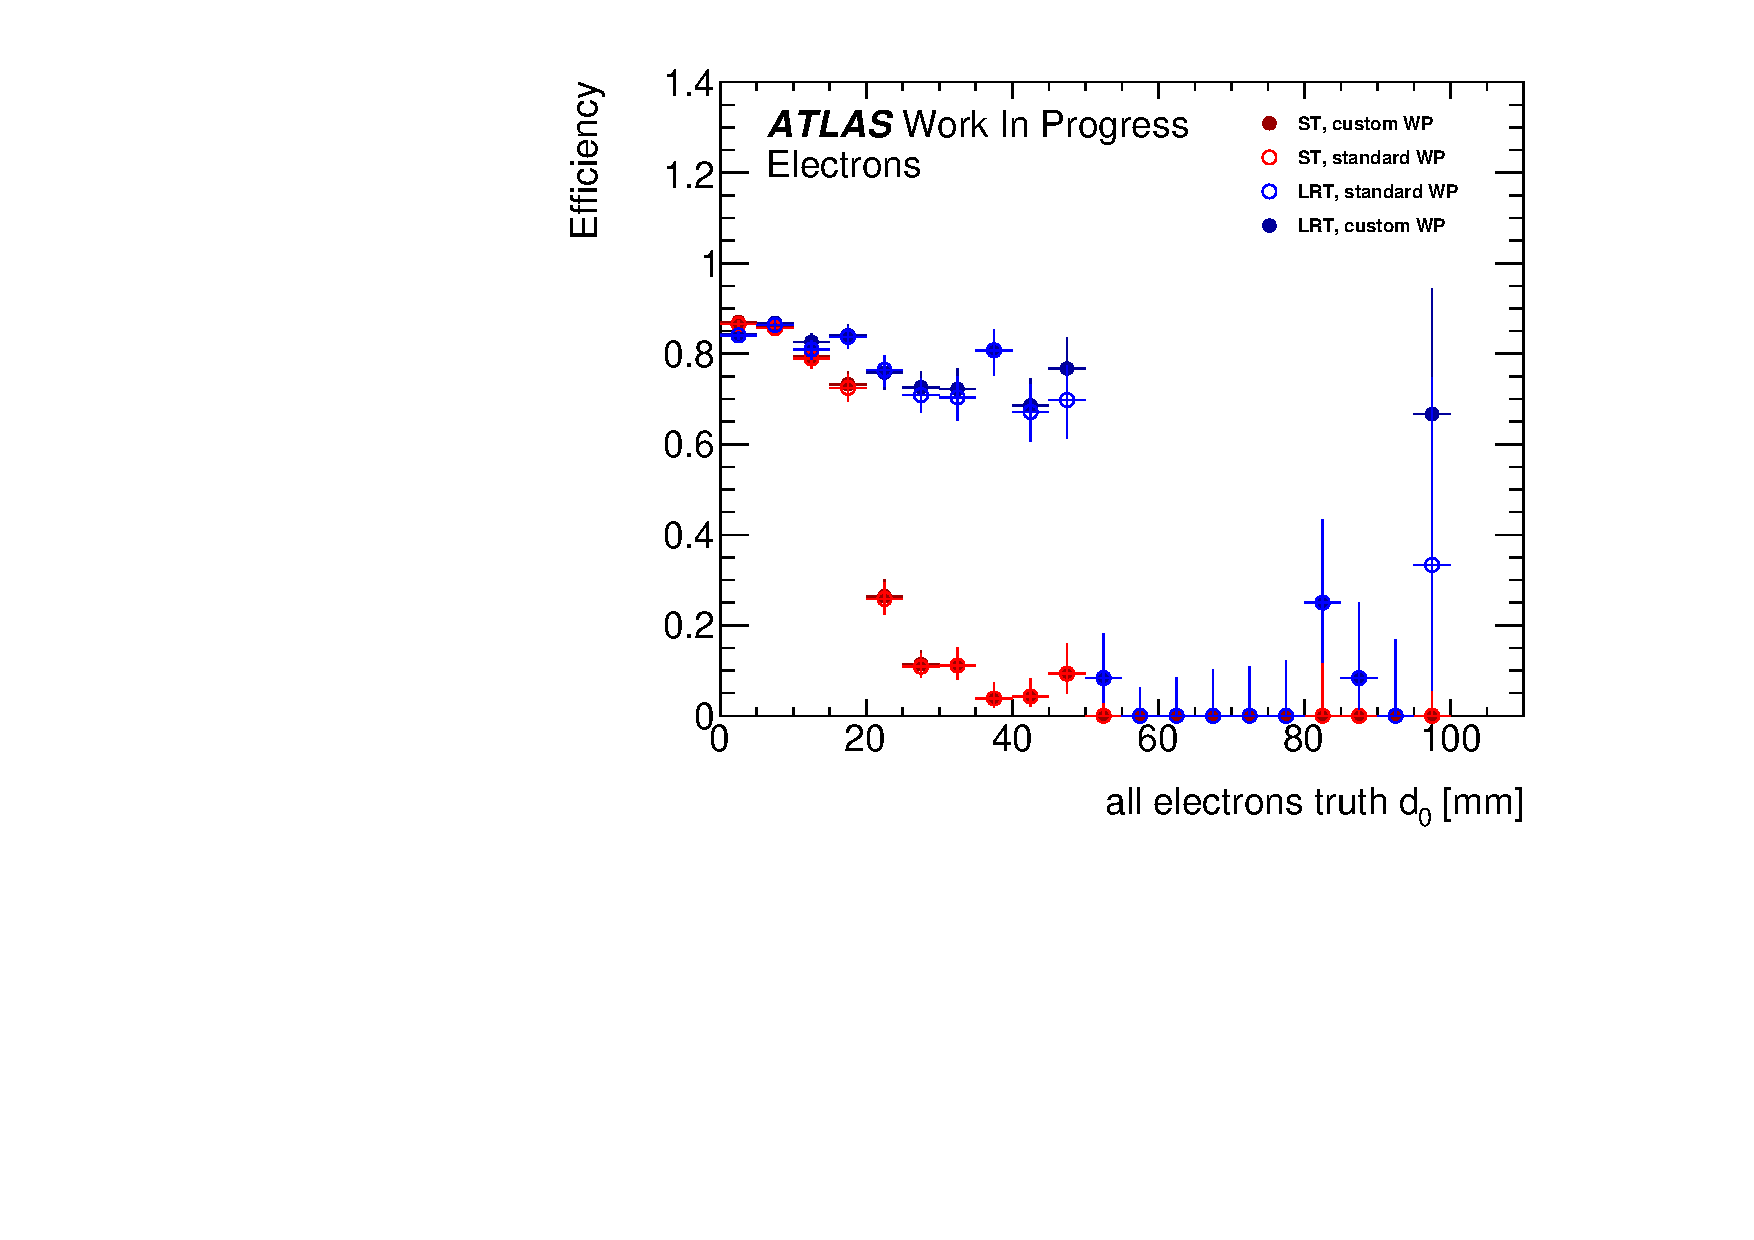
\includegraphics[width=.48\textwidth]{figures/EventReconstruction/wp_e_d0_all_wip.pdf}
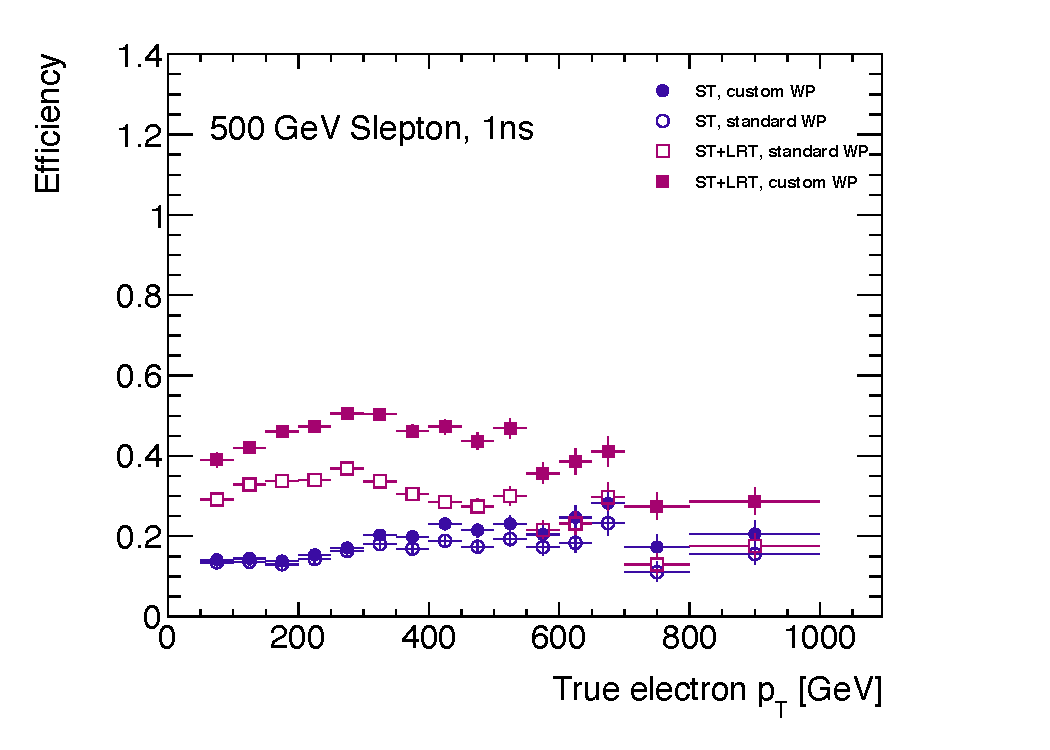
\includegraphics[width=.48\textwidth]{figures/EventReconstruction/wp_e_pt_all_wip.pdf}
\caption{Muon identification efficiency with modified criteria. Left is efficiency vs $d_{0}$ and right is efficiency as a function of $p_{T}$. The red denotes reconstruction with Standard Tracking (ST), and the blue with Large Radius Tracking (LRT), and the filled in circles use the modified identification working point. \todo{Needs update when available}}
\label{fig:cust_elec_eff}
\end{figure}




\section{Isolation}

In this analysis, both muons and electrons are required to be isolated to reduce background from heavy flavor decays. That is, they are not expected to be surrounded by much other activity from the hard scatter in either the Inner Detector or Calorimeters. Isolation is generally measured in terms as the scalar sum of energy in a radius $\Delta R = \sqrt{(\Delta \eta)^2 + (\Delta \phi)^2}$ around the lepton. Track based isolations are called $p_{T}^{\textrm{varcone}}$ and calorimeter based isolations called $E_{T}^{\textrm{topocone}}$. 

For example, the track-based isolation called $p_{T}^{\textrm{varcone30}}$ is the scalar sum of the transverse momenta of tracks with $p_{T} > 1 \GeV$ in a cone of $\Delta R = \textrm{min}(10 \GeV/p_{T}^{\ell}, 0.3)$, then a value is selected to determine what should be considered ``isolated''. Whereas the calorimeter-based isolation just counts the energy in a specified \dR, not as a function of the \pt of the particle. Isolation working points are then centrally defined as a combination of cuts on the track-based and calorimeter-based isolation. 

These definitions are much simpler for muons than for electrons. Electrons are very likely to emit bremsstrahlung radiation as they traverse the inner detector and those photons can then convert back into electrons. The tracks from these secondary particles are considered part of the electron's \pT. Furthermore, the electron leaves its own energy deposit in the \ac{EM} calorimeter and this energy must be subtracted from the $E_{T}^{\textrm{topocone}}$ calculation.


In this analysis we use the following working points \todo{grab isolation requirements from INT when finalized}


\section{Overlap Removal}
Each of the reconstruction chains described above, as well as those to reconstruction $\tau$ leptons, jets, and other physics objects used in \ac{ATLAS}, are run simultaneously. This means that the same track or cluster can be used to reconstruct two different types of physics objects. An iterative process of \ac{OR} is used to remove such artifacts. Overlap removal is performed on baseline objects, further described in \autoref{chap:event-selection}, which only pass identification and a loose \pt cut. 

Electrons $\dR < 0.01$ from a muon are removed to suppress contributions from muon bremsstrahlung radiation. Then, any baseline jet residing within $\Delta R < 0.2$ of a baseline electron is removed.  Baseline electrons with $E_{T}<50$~\GeV\ ($E_{T}>50$~\GeV) within $\Delta R < 0.4$ ($\Delta R < \mathrm{min}(0.4,0.04+10$~\GeV$/\pt)$) of any remaining jet are removed. The overlap removal procedure between muon and jet candidates is designed to remove muons that may originate from the decay of hadrons, with the overlapping jet being retained. Nearby jets may also occur as a result of high-\pt\ bremsstrahlung, in which case the jet should be removed and the muon retained. Such jets are removed if they reside within $\Delta R < 0.2$ of a baseline muon and have less than three matched inner detector tracks. Muons are removed if they reside within either $\Delta R < 0.4$ or $\Delta R < \mathrm{min}(0.4,0.04+10$~\GeV$/\pt)$ of any remaining jet, following the same \pt-dependent criteria as outlined for electrons above.




\cleardoublepage 

%----------------------------------------------------------------------------------------
\ctparttext{}
\part{Search for Displaced Leptons}

\cleardoublepage 

%----------------------------------------------------------------------------------------
\ctparttext{}
\part{Conclusions}

\cleardoublepage 



%----------------------------------------------------------------------------------------
%	THESIS CONTENT - APPENDICES
%----------------------------------------------------------------------------------------

\appendix

\part{Appendix} % New part of the thesis for the appendix

% Appendix A

\chapter{Appendix Test}

%----------------------------------------------------------------------------------------

\lipsum[13-14]

%----------------------------------------------------------------------------------------

\section{Appendix Section Test}
\lipsum[15]

\graffito{More dummy text}
\lipsum[16]

%----------------------------------------------------------------------------------------

\section{Another Appendix Section Test}
\lipsum[17]

\begin{table}
\myfloatalign
\begin{tabularx}{\textwidth}{Xll} \toprule
\tableheadline{labitur bonorum pri no} & \tableheadline{que vista}
& \tableheadline{human} \\ \midrule
fastidii ea ius & germano &  demonstratea \\
suscipit instructior & titulo & personas \\
\midrule
quaestio philosophia & facto & demonstrated \\
\bottomrule
\end{tabularx}
\caption[Autem usu id]{Autem usu id.}
\label{tab:moreexample}
\end{table}

\lipsum[18]

There is also a useless Pascal listing below: \autoref{lst:useless}.

\begin{lstlisting}[float=b,language=Pascal,frame=tb,caption={A floating example (\texttt{listings} manual)},label=lst:useless]
for i:=maxint downto 0 do
begin
{ do nothing }
end;
\end{lstlisting} % Appendix A
%% Appendix X

\chapter{Appendix Title}

%----------------------------------------------------------------------------------------

% Content begins here % Appendix B - empty template

%----------------------------------------------------------------------------------------
%	POST-CONTENT THESIS PAGES
%----------------------------------------------------------------------------------------

\cleardoublepage% Bibliography

\label{app:bibliography} % Reference the bibliography elsewhere with \autoref{app:bibliography}

\manualmark % Work-around to have small caps also here in the headline
\markboth{\spacedlowsmallcaps{\bibname}}{\spacedlowsmallcaps{\bibname}} % Work-around to have small caps also
%\phantomsection
\refstepcounter{dummy}

\addtocontents{toc}{\protect\vspace{\beforebibskip}} % Place the bibliography slightly below the rest of the document content in the table of contents
\addcontentsline{toc}{chapter}{\tocEntry{\bibname}}

\printbibliography % Bibliography

\cleardoublepage% Declaration

\refstepcounter{dummy}
\pdfbookmark[0]{Declaration}{declaration} % Bookmark name visible in a PDF viewer

\chapter*{Declaration} % Declaration section text

\thispagestyle{empty}

Put your declaration here.
\bigskip
 
\noindent\textit{\myLocation, \myTime}

\smallskip

\begin{flushright}
\begin{tabular}{m{5cm}}
\\ \hline
\centering\myName \\
\end{tabular}
\end{flushright}
 % Declaration

\cleardoublepage% Colophon (a brief description of publication or production notes relevant to the edition)

\pagestyle{empty}

\hfill

\vfill

\pdfbookmark[0]{Colophon}{colophon}

\section*{Colophon}

This document was typeset using the typographical look-and-feel \texttt{classicthesis} developed by Andr\'e Miede. The style was inspired by Robert Bringhurst's seminal book on typography ``\emph{The Elements of Typographic Style}''. \texttt{classicthesis} is available for both \LaTeX\ and \mLyX: 

\begin{center}
\url{https://bitbucket.org/amiede/classicthesis/}
\end{center}

\noindent Happy users of \texttt{classicthesis} usually send a real postcard to the author, a collection of postcards received so far is featured here: 

\begin{center}
\url{http://postcards.miede.de/}
\end{center}
 
\bigskip

\noindent\finalVersionString % Colophon

%----------------------------------------------------------------------------------------

\end{document}
